\documentclass[spanish,a4paper,11pt,twoside]{report}

%%%%%%%%%%%%%%%%%%%%%%%%%%%%%%%%%%%%%%%%%%%%%%%%%%%%%%%%%%%%%%%%%%%%%%%%%%%%%%%
\usepackage[dvips]{graphicx}
\usepackage[dvips]{epsfig}
\usepackage[latin1]{inputenc}
\usepackage[spanish]{babel}
\usepackage{alltt}
\usepackage{algorithm}
\usepackage{algorithmic}
\usepackage{multirow}

%%%%%%%%%%%%%%%%%%%%%%%%%%%%%%%%%%%%%%%%%%%%%%%%%%%%%%%%%%%%%%%%%%%%%%%%%%%%%%%

\newcommand{\SONY}{{\sc Sony}}
\newcommand{\MICROSOFT}{{\sc Microsoft}}
\newcommand{\GCC}{\textsf{\textsc{G}CC}}
\newcommand{\INTEL}{\textsf{\textsc{I}ntel}}

%%% Traducimos el pseudocodigo
\renewcommand{\algorithmicwhile}{\textbf{mientras}}
\renewcommand{\algorithmicend}{\textbf{fin}}
\renewcommand{\algorithmicdo}{\textbf{hacer}}
\renewcommand{\algorithmicif}{\textbf{si}}
\renewcommand{\algorithmicthen}{\textbf{entonces}}
\renewcommand{\algorithmicrepeat}{\textbf{repetir}}
\renewcommand{\algorithmicuntil}{\textbf{hasta que}}
\renewcommand{\algorithmicelse}{\textbf{en otro caso}}
\renewcommand{\algorithmicfor}{\textbf{para}}

%\newcommand{\RETURN}{\textbf{retornar} }
\newcommand{\RET}{\STATE \textbf{retornar} }
\newcommand{\TO}{\textbf{hasta} }
\newcommand{\AND}{\textbf{y} }
\newcommand{\OR}{\textbf{o} }

%%%%%%%%%%%%%%%%% Creamos un entorno para listar c�digo fuente %%%%%%%%%%%%%%%
\newenvironment{sourcecode}
{\begin{list}{}{\setlength{\leftmargin}{1em}}\item\scriptsize\bfseries}
{\end{list}}

\newenvironment{littlesourcecode}
{\begin{list}{}{\setlength{\leftmargin}{1em}}\item\tiny\bfseries}
{\end{list}}

\newenvironment{summary}
{\par\noindent\begin{center}\textbf{Abstract}\end{center}\begin{itshape}\par\noindent}
{\end{itshape}}

\newenvironment{keywords}
{\begin{list}{}{\setlength{\leftmargin}{1em}}\item[\hskip\labelsep \bfseries Keywords:]}
{\end{list}}

\newenvironment{palabrasClave}
{\begin{list}{}{\setlength{\leftmargin}{1em}}\item[\hskip\labelsep \bfseries Palabras clave:]}
{\end{list}}


%%%%%%%%%%%%%%%%%%%%%%%%%%%%%%%%%%%%%%%%%%%%%%%%%%%%%%%%%%%%%%%%%%%%%%%%%%%%%%%
% Format
%%%%%%%%%%%%%%%%%%%%%%%%%%%%%%%%%%%%%%%%%%%%%%%%%%%%%%%%%%%%%%%%%%%%%%%%%%%%%%%

%%\topmargin -4 mm
%\topmargin -21 mm
%\headheight 10 mm
%\headsep 10 mm

%\textheight 229 mm
%\textheight 246 mm

%\oddsidemargin -5.4 mm
%\evensidemargin -5.4 mm
\oddsidemargin 5 mm
\evensidemargin 5 mm

%\oddsidemargin -3 mm
%\evensidemargin -3 mm

%\textwidth 17 cm
\textwidth 15 cm
%\columnsep 10 mm

\input{amssym.def}

%%%%%%%%%%%%%%%%%%%%%%%%%%%%%%%%%%%%%%%%%%%%%%%%%%%%%%%%%%%%%%%%%%%%%%%%%%%%%%%

\begin{document}

%%%%%%%%%%%%%%%%%%%%%%%%%%%%%%%%%%%%%%%%%%%%%%%%%%%%%%%%%%%%%%%%%%%%%%%%%%%%%%%
% First Page 
%%%%%%%%%%%%%%%%%%%%%%%%%%%%%%%%%%%%%%%%%%%%%%%%%%%%%%%%%%%%%%%%%%%%%%%%%%%%%%%

\pagestyle{empty}
\thispagestyle{empty}


\newcommand{\HRule}{\rule{\linewidth}{1mm}}
\setlength{\parindent}{0mm}
\setlength{\parskip}{0mm}
\vspace*{\stretch{1}}

\begin{center}
\includegraphics[width=0.2\textwidth]{images/logotipo-secundario-ULL}\\[0.25cm]
\end{center}

\HRule
\begin{flushright}
        {\Huge T�tulo} \\[2.5mm] 
        {\Huge Subt�tulo.} \\[2.5mm]
        {\Large \textit{Title in English} .} \\[5mm]
        {\Large Autor} \\[5mm]
        Dpto. Nombre del Departamento \\[5mm]
        Escuela T\'ecnica Superior de Ingenier\'{\i}a Inform\'atica \\[5mm]
        
        Trabajo de Fin de Grado \\
\end{flushright}
\HRule
\vspace*{\stretch{2}}
\begin{center}
  \Large La Laguna, \today 
\end{center}

\setlength{\parindent}{5mm}

%%%%%%%%%%%%%%%%%%%%%%%%%%%%%%%%%%%%%%%%%%%%%%%%%%%%%%%%%%%%%%%%%%%%%%%%%%%%%%%
% Signature page (add the official stamp)
%%%%%%%%%%%%%%%%%%%%%%%%%%%%%%%%%%%%%%%%%%%%%%%%%%%%%%%%%%%%%%%%%%%%%%%%%%%%%%%
%\newpage
\cleardoublepage
\thispagestyle{empty}

D. {\bf Nombre Apellido1 Apellido2}, con N.I.F. 12.345.678-X 
profesor
Titular de Universidad 
adscrito al Departamento 
de Nombre del Departamento 
de la Universidad de La Laguna

\bigskip
\bigskip
\bigskip
\bigskip
\bigskip
{\bf C E R T I F I C A}

\bigskip
\bigskip
\bigskip
Que la presente memoria titulada:

\bigskip
``{\it Titulo del Trabajo.}''

\bigskip
\bigskip
\bigskip

\noindent ha sido realizada bajo su direcci�n por D. {\bf Nombre Apellido1 Apellido2},
con N.I.F. 12.345.678-X.

\bigskip
\bigskip

Y para que as� conste, en cumplimiento de la legislaci�n vigente y a los efectos
oportunos firman la presente en La Laguna a \today 

\cleardoublepage
%%%%%%%%%%%%%%%%%%%%%%%%%%%%%%%%%%%%%%%%%%%%%%%%%%%%%%%%%%%%%%%%%%%%%%%%%%%%%%%
\thispagestyle{empty}

{ \flushright

\begin{LARGE}
Agradecimientos
\end{LARGE}

\hspace{3mm}

\begin{large}


\hspace{3mm}
XXX

\hspace{3mm}
XXX


\hspace{3mm}
XXX


\hspace{3mm}
XXX


\end{large}

}

%%%%%%%%%%%%%%%%%%%%%%%%%%%%%%%%%%%%%%%%%%%%%%%%%%%%%%%%%%%%%%%%%%%%%%%%%%%%%%%
\cleardoublepage
\begin{abstract}
{\em 

El objetivo de este trabajo ha sido .... 
%
bla, bla, bla
%
bla, bla, bla
%
bla, bla, bla

}

\begin{palabrasClave}
Palabra reservada1, Palabra reservada2, ...
\end{palabrasClave}

\end{abstract}
%%%%%%%%%%%%%%%%%%%%%%%%%%%%%%%%%%%%%%%%%%%%%%%%%%%%%%%%%%%%%%%%%%%%%%%%%%%%%%%

%%%%%%%%%%%%%%%%%%%%%%%%%%%%%%%%%%%%%%%%%%%%%%%%%%%%%%%%%%%%%%%%%%%%%%%%%%%%%%%
\cleardoublepage
\begin{summary}
{\em 

Here should be the abstract in a foreing language...

}

\begin{keywords}
Keyword1, Keyword2, Keyword2, ...
\end{keywords}

\end{summary}
%%%%%%%%%%%%%%%%%%%%%%%%%%%%%%%%%%%%%%%%%%%%%%%%%%%%%%%%%%%%%%%%%%%%%%%%%%%%%%%

%%%%%%%%%%%%%%%%%%%%%%%%%%%%%%%%%%%%%%%%%%%%%%%%%%%%%%%%%%%%%%%%%%%%%%%%%%%%%%%
\newpage{\pagestyle{empty}\cleardoublepage}
\thispagestyle{empty}

%%%%%%%%%%%%%%%%%%%%%%%%%%%%%%%%%%%%%%%%%%%%%%%%%%%%%%%%%%%%%%%%%%%%%%%%%%%%%%%


\pagestyle{myheadings} %my head defined by markboth or markright
% No funciona bien \markboth sin "twoside" en \documentclass, pero al
% ponerlo se dan un mont�n de errores de underfull \vbox, con lo que no se
% ha puesto.
\markboth{Nombre del alumno}{T�tulo del proyecto}

%%%%%%%%%%%%%%%%%%%%%%%%%%%%%%%%%%%%%%%%%%%%%%%%%%%%%%%%%%%%%%%%%%%%%%%%%%%%%%%
%Numeracion en romanos
\renewcommand{\thepage}{\roman{page}}
\setcounter{page}{1}

%%%%%%%%%%%%%%%%%%%%%%%%%%%%%%%%%%%%%%%%%%%%%%%%%%%%%%%%%%%%%%%%%%%%%%%%%%%%%%%

\tableofcontents

%%%%%%%%%%%%%%%%%%%%%%%%%%%%%%%%%%%%%%%%%%%%%%%%%%%%%%%%%%%%%%%%%%%%%%%%%%%%%%%
\newpage{\pagestyle{empty}\cleardoublepage}

\listoffigures

%%%%%%%%%%%%%%%%%%%%%%%%%%%%%%%%%%%%%%%%%%%%%%%%%%%%%%%%%%%%%%%%%%%%%%%%%%%%%%%
\newpage{\pagestyle{empty}\cleardoublepage}

\listoftables

%%%%%%%%%%%%%%%%%%%%%%%%%%%%%%%%%%%%%%%%%%%%%%%%%%%%%%%%%%%%%%%%%%%%%%%%%%%%%%%
\newpage{\pagestyle{empty}\cleardoublepage}

%%%%%%%%%%%%%%%%%%%%%%%%%%%%%%%%%%%%%%%%%%%%%%%%%%%%%%%%%%%%%%%%%%%%%%%%%%%%%%%
%Numeracion a partir del capitulo I
\renewcommand{\thepage}{\arabic{page}}
\setcounter{page}{1}


\chapter{Introducci�n}
\label{chapter:intro}

%%%%%%%%%%%%%%%%%%%%%%%%%%%%%%%%%%%%%%%%%%%%%%%%%%%%%%%%%%%%%%%%%%%%%%%%%%%%%
% Chapter 1: Introducci�n 
%%%%%%%%%%%%%%%%%%%%%%%%%%%%%%%%%%%%%%%%%%%%%%%%%%%%%%%%%%%%%%%%%%%%%%%%%%%%%%%

%---------------------------------------------------------------------------------
\section{Antecedentes y estado actual del tema}
\label{1:sec:1}

La World Wide Web esta sujeta a un cambio continuo. La llegada de HTML5, la creciente importancia de AJAX y de la 
programaci\'on en el lado del cliente, las nuevas fronteras de la Web Sem\'antica, la explosi\'on de las redes 
sociales as\'{\i} como la llegada de las redes sociales federadas son ejemplos de esta tendencia general. 
Las aplicaciones web parecen evolucionar hacia entornos cada vez m\'as ricos y flexibles en los que los usuarios 
pueden acceder con facilidad a los documentos, publicar contenido, escuchar m\'usica, ver v\'{\i}deos, realizar dibujos
e incluso jugar usando un navegador. Esta nueva clase de software ubicuo no cesa de ganar \textit{momentum} y promueve nuevas 
formas de interacci\'on y cooperaci\'on.
\bigskip

Dentro del \'ambito educativo tambi\'en se ha vivido una revoluci\'on, en forma y contenido, de impartir ense�anza.
En Internet se puede encontrar, cada vez con m\'as facilidad, contenidos de cualquier disciplina en m\'ultiples
formatos: blogs, videotutoriales, presentaciones, ejercicios resueltos, etc.

Tambi\'en est\'an teniendo mucho \'exito las plataformas de aprendizaje virtual ofreciendo, adem\'as de conocimiento 
sin la necesidad de estar f\'{\i}sicamente presente en un aula, una serie de recompensas y medallas por ir obteniendo
logros. Esta metodolog\'{\i}a se denomina {\bfseries Gamificaci\'on} y est\'a teniendo un impacto muy positivo en los usuarios
de estas plataformas, ya que los anima a seguir usando estas herramientas de conocimiento.
\bigskip

Otro tipo de plataforma de aprendizaje virtual m\'as orientada a universidades e institutos es {\bfseries Moodle}. Est\'a implamantada
en numerosos centros de todo el planeta. Es el complemento perfecto para enriquecer las ense�anzas impartidas f\'{\i}sicamente
con cuestionarios autoevaluativos y compartici\'on de recursos adicionales. Adem\'as, facilita numerosas tareas a los docentes como 
la correcci\'on y calificaci\'on de ejercicios.

Sin embargo, esta plataforma s\'olo se limita a la evaluaci\'on de cuestiones triviales. Para la correci\'on de preguntas
propias de las ramas de Ingenier\'{\i}a, como pueden ser la implementaci\'on de c\'odigo, es necesaria la figura del profesor para
evaluar dichas tareas.

Otro problema que presenta es su dif\'{\i}cil portabilidad. Estamos hablando de un tipo de plataforma que sigue un
esquema {\bfseries cliente-servidor}, que no es f\'acilmente migrable a otras m\'aquinas.
\bigskip

Estas desventajas se ven resueltas con la {\bfseries Aplicaci\'on para la Elaboraci\'on y Despliegue de Cuestionarios} que se presentar\'a
en esta memoria.

%---------------------------------------------------------------------------------
\section{�Qu\'e es RuQL?}
\label{1:sec:2}

Esta aplicaci\'on de generaci\'on y despliegue de cuestionarios forma parte de una
gema de Ruby creada por \href{http://www.armandofox.com/geek}{Armando Fox} denominada 
\href{http://github.com/saasbook/ruql}{'Ruby-based Quiz Generator and DSL'} (RuQL).

Inicialmente, esta gema permit\'{\i}a generar un cuestionario partiendo de un fichero {\bfseries Ruby}, 
donde se redactaban las preguntas y respuestas haciendo uso de un {\bfseries DSL}.

Pose\'{\i}a una serie de \textit{renderers} que permit\'{\i}an generar los cuestionario en los siguientes formatos:
\begin{itemize}
  \item \href{http://code.edx.org/}{Open EdX}: formato \textit{open source} listo para importar en plataformas de aprendizaje online como {\bfseries EdX}.
  \item Versi\'on HTML 5 imprimible: lista para ser impresa y rellenada por los usuarios.
  Se le pod\'{\i}a pasar como argumento el path de una hoja de estilo para incorporarla al HTML de salida. Del mismo modo, se
  pod\'{\i}a especificar el path de un template predefinido por el profesor de modo que las preguntas se renderizaran en el mismo.
  \item \href{http://home.gna.org/auto-qcm}{AutoQCM}: formato listo para importar a {\bfseries AMC} (\textit{Auto Multiple Choice}), software libre
  que permite elaborar cuestionarios multirrespuesta.
\end{itemize}

Los tipos de preguntas que se pod\'{\i}an especificar eran:
\begin{itemize}
  \item {\bfseries Preguntas de completar}: en las cuales los usuarios deben rellenar los espacios en blanco. Admit\'{\i}a respuestas de tipo \textit{string} o
  \textit{regexp}. Si exist\'{\i}an m\'ultiples espacios para rellenar, se especificaban las respuestas en forma de \textit{array}, indicando adem\'as
  si el orden de las mismas influ\'{\i}a.
  Permit\'{\i}a adem\'as especificar respuestas falsas (\textit{distractors}) con una explicaci\'on de la misma, de modo que si el 
  alumno escrib\'{\i}a dicho \textit{distractor}, le apareciera la explicaci\'on de por qu\'e esa respuesta era incorrecta.
  
  [foto]
  
  \item {\bfseries Preguntas multirrespuesta con una  \'unica respuesta correcta}: las cl\'asicas preguntas tipo test. Se pod\'{\i}a aleatorizar el orden
  de las respuestas definido en el fichero de preguntas y asignarles explicaciones a los \textit{distractors} de manera individual o asignar una explicaci\'on
  general para todos los \textit{distractors}.
  
  [foto]
  
  Especificando adem\'as la opci\'on \textit{raw} a la pregunta, permit\'{\i}a incrustar dicho texto entre etiquetas \textless pre\textgreater \space HTML.
  
  [foto]
  
  \item {\bfseries Preguntas multirrespuesta con una  m\'ultiples respuestas correctas}: iguales a las preguntas multirrespuesta de opci\'on \'unica con la diferencia de 
  que existe m\'as de una respuesta correcta.
  
  [foto]
  
  \item {\bfseries Preguntas de verdadero o falso}: caso particular de las preguntas multirrespuesta de opci\'on \'unica.
  
  [foto]
  
\end{itemize}

Para todos los tipos de preguntas era posible especificar un comentario opcional que acompa�ar\'{\i}a al texto de la pregunta.

%---------------------------------------------------------------------------------
\section{Objetivos y actividades a realizar}
\label{1:sec:3}

Los objetivos propuestos para alcanzar en este Trabajo de Fin de Grado ha sido los siguientes:
\begin{itemize}
  \item Conocer, dominar y practicar con lenguajes y herramientas de desarrollo de aplicaciones web en el {\bfseries servidor}.
  \item Conocer, dominar y practicar con diferentes lenguajes y librer\'{\i}as en el {\bfseries cliente}.
  \item Conocer, practicar y dominar de herramientas de {\bfseries desarrollo dirigido por pruebas} (\textit{TDD}) en entornos web.
  \item Conocer, practicar y dominar diferentes lenguajes de marcas y de estilo.
  \item Conocer, practicar y dominar diferentes mecanismos de despliegue.
  \item Conocer, practicar y familiarizarse con diferentes mecanismos de seguridad, autentificaci\'on y autorizaci\'on.
  \item Conocer, practicar y dominar diferentes herramientas colaborativas y de {\bfseries control de versiones} (\textit{CVS}).
  \item Conocer, practicar y dominar {\bfseries metodolog\'{\i}as \'agiles} de desarrollo de software.
  \item Desarrollar una aplicaci\'on web para la elaboraci\'on y despliegue de cuestionarios.
\end{itemize}
\bigskip

Y las actividades a realizar en el mismo, tal cual est\'an descritas en la propuesta de {\bfseries Proyecto de Trabajo de Fin de Grado} firmada por 
el director y el alumno en la actividad 2 de la asignatura, son las que se describen a continuaci\'on:
\begin{itemize}
  \item Revisi\'on bibliogr\'afica.
  \item Realizaci\'on de una aplicaci\'on web en la que:
  \begin{itemize}
    \item Se proporciona soporte mediante una aplicaci\'on web a los procesos de evaluaci\'on.
    \item Se proporciona/extiende un {\bfseries Lenguaje de Dominio Espec\'{\i}fico} (\textit{DSL}) para la elaboraci\'on de cuestionarios.
    \item Se deber\'a considerar c\'omo resolver los problemas de seguridad asociados.
    \item Redacci\'on de la memoria.
  \end{itemize}
  \item Preparaci\'on de las presentaciones.
\end{itemize}



%---------------------------------------------------------------------------------
\section{Tecnolog\'{\i}a usada}
\label{1:sec:4}

Debido a que este Trabajo de Fin de Grado es una extensi\'on de una gema de {\bfseries Ruby}, se ha utilizado \'este como lenguaje de
programaci\'on.

Adem\'as, se ha hecho uso de un numeroso conjunto de gemas y de otras tecnolog\'{\i}as enumeradas a continuaci\'on:
\begin{itemize}
  \item HTML5: haciendo uso de funcionalidades como {\bfseries Local Storage} y {\bfseries Drag and Drop}.
  \item CSS3
  \item JavaScript
  \item \href{http://getbootstrap.com/}{Bootstrap}
  \item \href{https://jquery.com/}{jQuery}
  \item \href{http://xregexp.com/}{XRegExp}
  \item \href{http://www.mathjax.org/}{MathJax}
  \item \href{http://codemirror.net/}{CodeMirror}
  \item \href{https://visionmedia.github.io/mocha/}{Mocha}
  \item \href{http://chaijs.com/}{Chai}
  \item \href{https://karma-runner.github.io/0.12/index.html}{Karma}
  \item \href{http://www.sinatrarb.com/}{Sinatra}
  \item \href{https://github.com}{GitHub}
  \item \href{https://www.heroku.com/}{Heroku}
  \item \href{http://oauth.net/2/}{OAuth 2.0}
  \item \href{https://drive.google.com}{Google Drive}
  
  \bigskip
  [Iconos]
\end{itemize}


%------------------------------------------------------------------------------
\begin{figure}[!th]
\begin{center}
\includegraphics[width=0.5\textwidth]{images/arbolbinario.eps}
\caption{Ejemplo}
\label{fig:ArbolBinario}
\end{center}
\end{figure}
%------------------------------------------------------------------------------



%%%%%%%%%%%%%%%%%%%%%%%%%%%%%%%%%%%%%%%%%%%%%%%%%%%%%%%%%%%%%%%%%%%%%%%%%%%%%%%

\chapter{T�tulo del Cap�tulo Dos}
\label{chapter:dos}

%%%%%%%%%%%%%%%%%%%%%%%%%%%%%%%%%%%%%%%%%%%%%%%%%%%%%%%%%%%%%%%%%%%%%%%%%%%%%%%
% Chapter 2: Desarrollo
%%%%%%%%%%%%%%%%%%%%%%%%%%%%%%%%%%%%%%%%%%%%%%%%%%%%%%%%%%%%%%%%%%%%%%%%%%%%%%%

%++++++++++++++++++++++++++++++++++++++++++++++++++++++++++++++++++++++++++++++

En el cap\'{\i}tulo anterior se ha definido el Trabajo de Fin de Grado, especificado los objetivos y actividades
a desarrollar y mencionado las tecnolog\'{\i}as empleadas para su desarrollo. A continuaci\'on, se describir\'a 
la metodolog\'{\i}a de trabajo seguida y los problemas hallados durante el desarrollo junto con las soluciones
alcanzadas.

%++++++++++++++++++++++++++++++++++++++++++++++++++++++++++++++++++++++++++++++

\section{Metodolog\'{\i}a usada}
\label{sec:1}

La metodolog\'{\i}a que se ha seguido ha sido \textit{\'agil}: con iteraciones semanales en las que se defin\'{\i}an una serie
de tareas u objetivos y que se presentaban la siguiente semana. De este modo, con la entrega de prototipos funcionales
de la aplicaci\'on, se han ido testeando, corrigiendo y mejorando las funcionalidades, al mismo tiempo que detectando 
problemas no contemplados en las fases previas de dise�o. 
\bigskip

Esta metodolog\'{\i}a, adem\'as, ha propiciado la generaci\'on de ideas que se han traducido en nuevas caracter\'{\i}sticas.


%---------------------------------------------------------------------------------
\section{Problemas encontrados y soluciones}
\label{sec:2}

A continuaci\'n se detallan los problemas encontrados durante la implementaci\'on del Trabajo de Fin de Grado y las soluciones
encontradas para los mismos.

\subsection{Entender el funcionamiento del c\'odigo de la gema}
\label{subsec:2.1}
\bigskip

{\normalsize {\bfseries Soluci\'on}}

Leer la documentaci\'on de la gema, generar cuestionarios de pruebas y estudiar el c\'odigo fuente.

\subsection{Corregir tests y funcionalidades de la gema}
\label{subsec:2.2}
\bigskip

{\normalsize {\bfseries Soluci\'on}}

Tras realizar el correspondiente \textit{fork} en GitHub para empezar a implementar mis modificaciones, ejecut\'e los tests de la 
gema original para comprobar la ausencia de fallos. Al finalizar, algunos tests fallaron por lo que decid\'{\i} corregirlos. Del 
mismo modo, algunas gemas de testing existentes en el Gemfile presentaban incompatibilidades con las nuevas versiones de Ruby, por
lo que tambi\'en se corrig\'{\i}o.
\bigskip

Del mismo modo, las siguientes funcionalidades de la gema fueron corregidas ya que no funcionaban correctamente:
\begin{itemize}
  \item La opci\'on que permite indicar si el orden de las respuestas en las preguntas de completar espacios en blaco importa o no.
  \item La opci\'on de a�adir comentarios opcionales a los textos de las preguntas.
  \item La opci\'on \textit{raw} que permite incrustar el texto de las preguntas entre etiquetas \textless pre\textgreater \space HTML.
  \item La opci\'on de explicaci\'on global para todos los \textit{distractors} no funcionaba.
\end{itemize}



%%%%%%%%%%%%%%%%%%%%%%%%%%%%%%%%%%%%%%%%%%%%%%%%%%%%%%%%%%%%%%%%%%%%%%%%%%%%%%%
\newpage{\pagestyle{empty}\cleardoublepage}
\thispagestyle{empty}

\chapter{T�tulo del Cap�tulo Tres}
\label{chapter:tres}

%%%%%%%%%%%%%%%%%%%%%%%%%%%%%%%%%%%%%%%%%%%%%%%%%%%%%%%%%%%%%%%%%%%%%%%%%%%%%%%
% Chapter 3: Resultados
%%%%%%%%%%%%%%%%%%%%%%%%%%%%%%%%%%%%%%%%%%%%%%%%%%%%%%%%%%%%%%%%%%%%%%%%%%%%%%%

%++++++++++++++++++++++++++++++++++++++++++++++++++++++++++++++++++++++++++++++


Tras explicar en el cap\'{\i}tulo anterior la metodolog\'{\i}a empleada, los problemas encontrados
durante la fase de desarrollo e implementaci\'on y las soluciones halladas, a continuaci\'on se
detallar\'an todos los resultados obtenidos.

%++++++++++++++++++++++++++++++++++++++++++++++++++++++++++++++++++++++++++++++
\section{Enriquecimiento del DSL original}
\label{3:sec1}

Se han extendido las funcionalidades originales del DSL de la gema. A continuaci\'on se enumerar\'an
todas las nuevas caracter\'{\i}sticas:

\begin{itemize}
  \item 
  \item 
  \item 
  \item 
\end{itemize}

%++++++++++++++++++++++++++++++++++++++++++++++++++++++++++++++++++++++++++++++
\section{Creaci\'on del renderer HTMLForm}
\label{3:sec2}

Este renderer permite generar un documento HTML5 con un formulario en el que se encontran todas las
preguntas listas para ser completadas desde el navegador.

%++++++++++++++++++++++++++++++++++++++++++++++++++++++++++++++++++++++++++++++
\section{Tercer apartado de este capitulo}
\label{:sec3}


%%%%%%%%%%%%%%%%%%%%%%%%%%%%%%%%%%%%%%%%%%%%%%%%%%%%%%%%%%%%%%%%%%%%%%%%%%%%%%%

\chapter{T�tulo del Cap�tulo Cuatro}
\label{chapter:cuatro}

%%%%%%%%%%%%%%%%%%%%%%%%%%%%%%%%%%%%%%%%%%%%%%%%%%%%%%%%%%%%%%%%%%%%%%%%%%%%%%%
% Chapter 4 : Título del Capítulo cuatro
%%%%%%%%%%%%%%%%%%%%%%%%%%%%%%%%%%%%%%%%%%%%%%%%%%%%%%%%%%%%%%%%%%%%%%%%%%%%%%%

%++++++++++++++++++++++++++++++++++++++++++++++++++++++++++++++++++++++++++++++

En el capitulo ~\ref{chapter:intro} se describio bla, bla, bla.....




%%%%%%%%%%%%%%%%%%%%%%%%%%%%%%%%%%%%%%%%%%%%%%%%%%%%%%%%%%%%%%%%%%%%%%%%%%%%%%%
\newpage{\pagestyle{empty}\cleardoublepage}
\thispagestyle{empty}

\chapter{Conclusiones y trabajos futuros}
\label{chapter:Conclusiones}

%%%%%%%%%%%%%%%%%%%%%%%%%%%%%%%%%%%%%%%%%%%%%%%%%%%%%%%%%%%%%%%%%%%%%%%%%%%%%
% Chapter 5: Conclusiones y Trabajos Futuros 
%%%%%%%%%%%%%%%%%%%%%%%%%%%%%%%%%%%%%%%%%%%%%%%%%%%%%%%%%%%%%%%%%%%%%%%%%%%%%%%

%++++++++++++++++++++++++++++++++++++++++++++++++++++++++++++++++++++++++++++++

Este cap�tulo es obligatorio.
Toda memoria de Trabajo de Fin de Grado debe incluir unas conclusiones y unas 
l�neas de trabajo futuro 



%%%%%%%%%%%%%%%%%%%%%%%%%%%%%%%%%%%%%%%%%%%%%%%%%%%%%%%%%%%%%%%%%%%%%%%%%%%%%%%
\newpage{\pagestyle{empty}\cleardoublepage}
\thispagestyle{empty}

\chapter{Summary and Conclusions }
\label{chapter:ingles}

%%%%%%%%%%%%%%%%%%%%%%%%%%%%%%%%%%%%%%%%%%%%%%%%%%%%%%%%%%%%%%%%%%%%%%%%%%%%%
% Chapter 5: Conclusiones y Trabajos Futuros 
%%%%%%%%%%%%%%%%%%%%%%%%%%%%%%%%%%%%%%%%%%%%%%%%%%%%%%%%%%%%%%%%%%%%%%%%%%%%%%%

%++++++++++++++++++++++++++++++++++++++++++++++++++++++++++++++++++++++++++++++

Desde hace unos a�os hasta ahora, ha tenido lugar un enorme crecimiento de las \ceit{plataformas} de aprendizaje online. Cada vez
cuentan con m\'as adeptos y las instituciones de ense\~{n}anza saben que incorporarlas a sus sistemas educativos es clave
para ofrecer un servicio puntero y de calidad.

\'Esto es lo que se pretende con la herramienta obtenida tras la realizaci\'on de este Trabajo de Fin de Grado: que sea posible
su implantaci\'on dentro del marco acad\'emico de la Universidad de La Laguna, partiendo de la premisa de que nos estamos adentrando 
en una \'epoca en la que estas herramientas de aprendizaje online seguir\'an evolucionando y teniendo un papel importante en la educaci\'on.
\bigskip

En este trabajo se proporciona/extiende un \ceis{Lenguaje de Dominio Espec\'{\i}fico} (\cei{DSL}) para la \ceit{elaboraci\'on} y \ceit{evaluaci�n} de \ceit{cuestionarios} que ofrece varias ventajas 
con respecto a otras herramientas equivalentes:
\begin{enumerate}
  \item Portabilidad: la principal ventaja sobre plataformas como Moodle\cite{moodle}.
  \item Respuestas que pueden ser evaluadas mediante \ceit{expresiones regulares} extendidas.
  \item Respuestas que pueden ser evaluadas mediante \ceit{c\'odigo} arbitrario definido por el profesor.
  \item Generaci\'on de c\'odigo para diversas plataformas y formas de uso: generaci\'on de \ceit{HTML} \cei{standalone} para entrenamiento y retroalimentaci\'on del alumno, \ceit{XML} 
  para \ceit{edX}\cite{edx} y \ceit{AutoQCM} para \ceit{AMC}\cite{amc}.
  \item \ceit{Escalabilidad}: posibilidad de implantar soporte para cualquier otra plataforma o forma de uso que se desee mediante el uso de \ceit{renderers}.
  \item Generaci\'on de una \ceit{aplicaci\'on} \ceit{Sinatra} de \ceit{evaluaci\'on} completa con almacenamiento de ex\'amenes y datos en \ceis{Google Drive}. Una soluci\'on innovadora que
  facilita la gesti\'on de los mismo y evita tener que almacenar preguntas, respuestas, alumnos y calificaciones en bases de datos tradicionales junto con los problemas relacionados con su 
  manipulaci\'on y exportaci\'on a formatos m\'as \'utiles, como puede ser, las hojas de c\'alculo.
\end{enumerate}

Adem\'as, teniendo en cuenta aspectos \'eticos y legales, se hace uso de \ceis{OAuth} para delegar a \ceit{Google} la acci\'on de la autentificaci\'on. De este modo, se evitan problemas de brechas de 
seguridad como puede ser la suplantaci\'on de identidad o la exposici\'on de datos sensibles de los usuarios a terceras personas.
\bigskip

Para concluir, podemos afirmar que los objetivos han sido cumplidos, tanto los establecidos de la gu\'{\i}a docente de la asignatura junto con la adquisi\'on de las competencias generales y 
espec\'{\i}ficas como los marcados al comienzo de la asignatura. Sin embargo, el desarrollo no finaliza aqu\'{\i}. A\'un queda trabajo por realizar para poder garantizar un eficaz funcionamiento y 
rendimiento de esta herramienta. El estado final de la misma puede ser el punto de partida para pr\'oximos Trabajos de Fin de Grado.
\bigskip

As\'{\i} pues, las principales l\'{\i}neas de desarrollo a continuar ser\'{\i}an las enumeradas a continuaci\'on:
\begin{itemize}
  \item Resolver los problemas de \ceit{seguridad} relacionados con evaluar el c\'odigo escrito por los alumnos.
  \item Dar soporte a preguntas con respuestas de c\'odigo en otros \ceit{lenguajes de programaci\'on}.
  \item Ofrecer una alternativa de despliegue distinta a \ceit{Heroku}, como podr\'{\i}a ser un \ceit{servidor dedicado} ofrecido por la Universidad de
  La Laguna.
\end{itemize}


%%%%%%%%%%%%%%%%%%%%%%%%%%%%%%%%%%%%%%%%%%%%%%%%%%%%%%%%%%%%%%%%%%%%%%%%%%%%%%%
\newpage{\pagestyle{empty}\cleardoublepage}
\thispagestyle{empty}

\chapter{Presupuesto}
\label{chapter:Presupuesto}

%%%%%%%%%%%%%%%%%%%%%%%%%%%%%%%%%%%%%%%%%%%%%%%%%%%%%%%%%%%%%%%%%%%%%%%%%%%%%
% Chapter 6: Summary and Conlusions
%%%%%%%%%%%%%%%%%%%%%%%%%%%%%%%%%%%%%%%%%%%%%%%%%%%%%%%%%%%%%%%%%%%%%%%%%%%%%%%

%++++++++++++++++++++++++++++++++++++++++++++++++++++++++++++++++++++++++++++++

% Desde hace unos años hasta ahora, ha tenido lugar un enorme crecimiento de las \ceit{plataformas} de aprendizaje online. Cada vez
% cuentan con m\'as adeptos y las instituciones de ense\~{n}anza saben que incorporarlas a sus sistemas educativos es clave
% para ofrecer un servicio puntero y de calidad.

For some years to now, it has taken place a huge growth of the online learning platforms. This platforms are having more followers each time and
academic institutions know that include them to their educational systems is the key to offer a better quality service.

% \'Esto es lo que se pretende con la herramienta obtenida tras la realizaci\'on de este Trabajo de Fin de Grado: que sea posible
% su implantaci\'on dentro del marco acad\'emico de la Universidad de La Laguna, partiendo de la premisa de que nos estamos adentrando 
% en una \'epoca en la que estas herramientas de aprendizaje online seguir\'an evolucionando y teniendo un papel importante en la educaci\'on.
% \bigskip

That's what we except with our tool developed during the Final Degree Project: that it could be possible to install the tool within University of La Laguna learning system.
We're in a epoch which online learning tools are evolving and playing an important paper in the education.
\bigskip

% En este trabajo se proporciona/extiende un \ceis{Lenguaje de Dominio Espec\'{\i}fico} (\cei{DSL}) para la \ceit{elaboraci\'on} y \ceit{evaluación} de \ceit{cuestionarios} que ofrece varias ventajas 
% con respecto a otras herramientas equivalentes:
% \begin{enumerate}
% \item Portabilidad: la principal ventaja sobre plataformas como Moodle\cite{moodle}.
% \item Respuestas que pueden ser evaluadas mediante \ceit{expresiones regulares} extendidas.
% \item Respuestas que pueden ser evaluadas mediante \ceit{c\'odigo} arbitrario definido por el profesor.
% \item Generaci\'on de c\'odigo para diversas plataformas y formas de uso: generaci\'on de \ceit{HTML} \cei{standalone} para entrenamiento y retroalimentaci\'on del alumno, \ceit{XML} 
% para \ceit{EdX}\cite{edx} y \ceit{AutoQCM} para \ceit{AMC}\cite{amc}.
% \item \ceit{Escalabilidad}: posibilidad de implantar soporte para cualquier otra plataforma o forma de uso que se desee mediante el uso de \ceit{renderers}.
% \item Generaci\'on de una \ceit{aplicaci\'on} \ceit{Sinatra} de \ceit{evaluaci\'on} completa con almacenamiento de ex\'amenes y datos en \ceis{Google Drive}. Una soluci\'on innovadora que
% facilita la gesti\'on de los mismo y evita tener que almacenar preguntas, respuestas, alumnos y calificaciones en bases de datos tradicionales junto con los problemas relacionados con su 
% manipulaci\'on y exportaci\'on a formatos m\'as \'utiles, como puede ser, las hojas de c\'alculo.
% \end{enumerate}

This Final Degree Project provides and extends a Domain Specific Language (DSL) for the generation and evaluation of questionaries which offers several improvements regarding to other equivalents 
tools:
\begin{enumerate}
  \item Portability: the main advantage over other platforms like Moodle\cite{moodle}
  \item Answers that can be evaluated by extended regular expressions.
  \item Answers that can be evaluated by tests written by the teacher.
  \item Code generator for several platforms and ways of use: HTML standalone generator for students' training and feedback, XML for edX\cite{edx} and AutoQCM for AMC\cite{amc}.
  \item Scalability: possibility of introduce support for any other platform or way of use by the creation of renderers.
  \item Generation of a Sinatra application for a complete evaluation with exams and data storage in Google Drive. An innovation solution that makes the manage of them easier and it avoids has to 
store questions, answers, students and marks into a database and the handling and exportation to more useful formats like spreadsheets. 
\end{enumerate}

% Adem\'as, teniendo en cuenta aspectos \'eticos y legales, se hace uso de \ceis{OAuth} para delegar a \ceit{Google} la acci\'on de la autentificaci\'on. De este modo, se evitan problemas de brechas de 
% seguridad como puede ser la suplantaci\'on de identidad o la exposici\'on de datos sensibles de los usuarios a terceras personas.
% \bigskip

On the other hand, keeping in mind ethic and legal topics, we use OAuth to delegate the autentication to Google. This way, we avoid security bugs as the phishing or the exposure of sensitive 
information to third people.
\bigskip

% Para concluir, podemos afirmar que los objetivos han sido cumplidos, tanto los establecidos de la gu\'{\i}a docente de la asignatura junto con la adquisi\'on de las competencias generales y 
% espec\'{\i}ficas como los marcados al comienzo de la asignatura. Sin embargo, el desarrollo no finaliza aqu\'{\i}. A\'un queda trabajo por realizar para poder garantizar un eficaz funcionamiento y 
% rendimiento de esta herramienta. El estado final de la misma puede ser el punto de partida para pr\'oximos Trabajos de Fin de Grado.
% \bigskip

In conclusion, we can affirm that all the aims has been accomplish: the aims established in the teaching guide with the adquisition of general and specific competences and the aims established at the
beggining of the subject. However, the development hasn't finished here. Still there're some work to make for guarantee an effective running and performance of this tool. This tool's state can be
the starting point of another Final Degree Project.
\bigskip

% As\'{\i} pues, las principales l\'{\i}neas de desarrollo a continuar ser\'{\i}an las enumeradas a continuaci\'on:
% \begin{itemize}
%   \item Resolver los problemas de \ceit{seguridad} relacionados con evaluar el c\'odigo escrito por los alumnos.
%   \item Dar soporte a preguntas con respuestas de c\'odigo en otros \ceit{lenguajes de programaci\'on}.
%   \item Ofrecer una alternativa de despliegue distinta a \ceit{Heroku}, como podr\'{\i}a ser un \ceit{servidor dedicado} ofrecido por la Universidad de
%   La Laguna.
% \end{itemize}

So, the main development lines to continue will be the following:

\begin{itemize}
  \item Solve the security problem related with the student code evaluation in the server.
  \item Provide support to questions with answers written in another programming language.
  \item Provide a deployment alternative different to Heroku. It could be a dedicated server supplied by the University of La Laguna.
\end{itemize}

%%%%%%%%%%%%%%%%%%%%%%%%%%%%%%%%%%%%%%%%%%%%%%%%%%%%%%%%%%%%%%%%%%%%%%%%%%%%%%%

%%%%%%%%%%%%%%%%%%%%%%%%%%%%%%%%%%%%%%%%%%%%%%%%%%%%%%%%%%%%%%%%%%%%%%%%%%%%%%%
\newpage{\pagestyle{empty}\cleardoublepage}
\thispagestyle{empty}
\begin{appendix}

\chapter{T�tulo del Ap�ndice 1}
\label{appendix:1}
\section{T}
\label{Apendice1:T}

T\'erminos
\bigskip

Lenguaje de Dominio Espec\'{\i}fico (DSL)
\bigskip

Ruby
\bigskip

Sinatra
\bigskip

RuQL
\bigskip

Bootstrap
\bigskip

Open EdX
\bigskip

Renderer
\bigskip

Fork
\bigskip

Gema
\bigskip

HTML5
\bigskip

CSS3
\bigskip

Desarrollo Dirigido por Test (TDD)
\bigskip

Control de Versiones (CVS)
\bigskip

Metodolog\'{\i}a \'agil
\bigskip

GitHub
\bigskip

Template
\bigskip

Gemfile
\bigskip

Header
\bigskip

Footer
\bigskip

CSV
\bigskip

ERB
\bigskip

World Wide Web
\bigskip

Web semantica
\bigskip

AJAX
\bigskip

Moodle
\bigskip

Gamificacion
\bigskip

Cliente-Servidor
\bigskip

TDD
\bigskip

Framework
\bigskip

CDN
\bigskip

Lambda, Proc
\bigskip

Opal
\bigskip

WeBrick
\bigskip

Thin
\bigskip

\chapter{T�tulo del Ap�ndice 2}
\label{appendix:2}
El objetivo de esta gu\'{\i}a de usuario es proporcionar a los usuarios un ejemplo para la puesta a punto y ejecuci\'on de las 
funcionalidades implementadas en el gema RuQL durante el Trabajo de Fin de Grado.

%---------------------------------------------------------------------------------
\section{Instalaci\'on de la gema}
\label{Apendice2:instalacion}

Para instalar la \ceit{gema}, basta con ejecutar el siguiente comando:
\begin{verbatim}
[~]$ gem install ruql
\end{verbatim}

Si deseamos ejecutar la gema sin instalarla, debemos hacer lo siguiente:
\begin{itemize}
  \item Descargar el c\'odigo desde \ceit{GitHub}.
  \item Ejecutar el siguiente comando desde la ra\'{\i}z del proyecto:
  \begin{verbatim}
  [~]$ ruby -Ilib bin/ruql [argumentos]
  \end{verbatim}
\end{itemize}

% Poner tareas de Rake

Para consultar la ayuda sobre qu\'e argumentos opcionales recibe cada \ceit{renderer}, basta con escribir lo siguiente:
\begin{verbatim}
[~]$ ruql --help
\end{verbatim}
si tenemos la gema instalada en nuestra m\'aquina o
\begin{verbatim}
[~]$ ruby -Ilib bin/ruql --help
\end{verbatim}
si la ejecutamos desde el c\'odigo fuente.

Entre ellos destacan las opciones de a\~{n}adir hojas de estilo (\textit{-c}), JavaScripts (\textit{-j}) y especificar un propio \ceit{template} (\textit{-t}) de \ceis{ERB}.
Si se desea emplear un template propio, \'este debe contener una serie de variables obligatoriamente para que se inserten los recursos necesarios y el renderer funcione
correctamente. A continuaci\'on se muestra un ejemplo de template con dichas variables necesarias. Adem\'as, ser\'a posible a\~{n}adirle un \ceit{header} y un \ceit{footer} personalizado. 
De este modo no ser\'{\i}a necesario elaborar un template completamente nuevo cada vez. Para ello basta con indicarlo en nuestro fichero Ruby. Los m\'etodos \textit{head} y
\textit{foot} admiten tanto un path (escrito como un \ceis{s\'{\i}mbolo}) de donde se encuentre el \ceit{c\'odigo} \ceit{HTML} o un {\bfseries string} con el propio HTML:

\begin{lstlisting}
<html>
  <head>
    <meta charset="utf-8">
    <meta http-equiv="X-UA-Compatible" content="IE=edge">
    <meta name="viewport" content="width=device-width, initial-scale=1">
    <title><%= quiz.title %></title>
    <!-- Bootstrap CSS -->
    <%= @bootstrap_css %>
    <style type="text/css" media="all">
      /* Custom CSS */
      /* ...........*/
      /* Inputs size */
      <%= @sass %>
    </style>
    <!-- jQuery ContextMenu CSS -->
    <%= @context_menu_css %>
    <!-- Any CSS included by the user -->
    <%= @css_custom %>
    <!-- Mathjax -->
    <%= @mathjax %>
    <!-- CodeMirror -->
    <%= @codemirror %>
  </head>
  <body>
   <div class="container">
      <% if (quiz.get_header)%>
          <h3><%= quiz.title %></h3>
          <%= quiz.get_header %>
          <br></br>
      <% else %>
        <!-- HTML Code -->
      <% end %>
      <%= yield %>
      <% if (quiz.get_footer) %>
        <%= quiz.get_footer %>
        <br></br>
      <% else %>
        <!-- HTML Code -->
      <% end %>
    </div>
    <!-- #### JavaScripts #### -->
    <!-- jQuery -->
    <%= @jQuery %>
    <!-- Internationalization -->
    <%= @i18n %>
    <!-- Drag and Drop -->
    <%= @dragdrop %>
    <!-- XRegexp -->
    <%= @xregexp %>
    <!-- Form validation -->
    <%= @validation_js %>
    <!-- jQuery ContextMenu -->
    <%= @context_menu %>
    <!-- Any JavaScript included by the user -->
    <%= @js_custom %>
    <!-- CodeMirror object -->
    <%= @codemirror_object %>
    <!-- JavaScript for Bootstrap -->
    <%= @bootstrap_js %>
  </body>
</html>
\end{lstlisting}

Si no se especifica template, se mostrar\'a un HTML sin apenas estilo. El profesor se deber\'a encargar de adecuarlo a su gusto posteriormente. 

%---------------------------------------------------------------------------------
%---------------------------------------------------------------------------------
\section{HtmlForm renderer}
\label{Apendice2:htmlform}

A continuaci\'on veremos un ejemplo de \ceit{cuestionario} explicando las peculiaridades de cada tipo de pregunta:

El fichero \ceit{Ruby} debe comenzar de esta manera:
\begin{verbatim}
quiz 'Example quiz' do
  head :'examples/header.html'  # Opcional
  
  # Preguntas
  
  foot :'examples/footer.html'  # Opcional
end
\end{verbatim}
\bigskip

%---------------------------------------------------------------------------------
\subsection{Preguntas \ceit{FillIn}}
\label{subsec:Apendice2.1}

Para que el \ceit{renderer} genere las etiquetas \ceit{input}, se deben especificar tres guiones ('-') como m\'{\i}nimo. Si la cantidad es menor que tres, se mostrar\'an los guiones
en el cuestionario. Si queremos que se muestren m\'as de tres guiones seguidos, debemos escaparlos. Recuerda adem\'as que el n\'umero de guiones establecer\'a el largo del input.
\begin{verbatim}
tag = '<a href="www.google.es"></a> '
fill_in do
  text "<i>Example of escaped HTML and three hyphens not evaluated:</i><br> 
  #{escape(tag)}" + "is a \\-\\-\\- ---- " + '\-\-\-'
  answer /^link$/
end
\end{verbatim}
\bigskip

Ejemplo de pregunta con un \cei{distractor} y un comentario:
\begin{verbatim}
fill_in :points => 2 do
  text 'The visionary founder of Apple is --------'
  comment 'Question too easy'
  answer /^ste(ve|phen)\s+jobs #comment $/imx
  distractor /^steve\s+wozniak/i, :explanation => 'Almost, but not quite.'
end
\end{verbatim}
\bigskip

Ejemplo de pregunta con c\'odigo \ceit{LaTeX}:
\begin{verbatim}
fill_in do
  text %q{
    When x = 2, the solution of $\sqrt{3x+3}+(1+x)^2$ is:
    ----
  }
  answer 12
  distractor 11, :explanation => "Try again!"
end
\end{verbatim}
\bigskip

La respuesta a la pregunta puede ser una cadena, una expresi\'on regular, un n\'umero o un objeto \ceit{JavaScript}. En el caso de los tres primeros tipos de respuesta, se usar\'a
un \cei{Array} si hay m\'as de una respuesta en la pregunta.
\begin{verbatim}
fill_in do
  text 'The ---- brown fox jumped over the lazy ----'
  answer [/fox/, /dog/]
end
\end{verbatim}
\bigskip

Se puede usar la opci\'on \textit{order} para especificar si las respuestas dadas se corresponden con el orden dado en la pregunta. Por defecto est\'a a {\bfseries true}.
\begin{verbatim}
fill_in do
  text 'The ---- brown fox jumped over the lazy ----'
  answer [/fox/, /dog/], :order => false
end
\end{verbatim}

{\bfseries NOTA}: en caso de especificar en el Array dos respuestas iguales para dos huecos diferentes, forzosamente es necesario especificar \textit{order} a {\bfseries true}.
\bigskip

Tambi\'en se pueden escribir este tipo de preguntas de dos formas m\'as compactas:

Esta primera forma permite colocar la respuesta al lado de los guiones. S\'olo se admiten respuestas de tipo \cei{String}.
\begin{verbatim}
fill_in do
  text 'The three stooges are -----{larry}, ----{moe}, and -----{curly}.'
end
\end{verbatim}
\bigskip

Esta otra forma permite asociar las respuestas con una clave, que la definiremos en un \ceis{Hash} que se pasar\'a como respuesta.
\begin{verbatim}
fill_in do
  text "The capital of Tenerife is -----{:santa} Cruz de --------{:tenerife}"
  answer :santa => /Santa/i, :tenerife => /Tenerife/i
end
\end{verbatim}
\bigskip

Por \'ultimo, tenemos las respuestas de tipo {\bfseries objeto JavaScript}. La opci\'on \textit{order} debe ser siempre {\bfseries true}:
\begin{verbatim}
fill_in do
  text %q{
    Diga dos numeros x = ---- e  y = ---- que multiplicados den 100
  }
  answer JavaScript.new(%q{result = function(x,y) { return (x * y === 100); }})
end
\end{verbatim}

%---------------------------------------------------------------------------------
\subsection{Preguntas \ceit{Drag and Drop} FillIn}
\label{subsec:Apendice2.2}

Son muy similares a las preguntas FillIn normales. S\'olo admiten respuestas de tipo \textit{String} pero admiten los mismos par\'ametros opcionales.
\begin{verbatim}
drag_drop_fill_in do
  text 'The ---- brown fox jumped over the lazy ----'
  answer ['fox', 'dog']
end
\end{verbatim}

%---------------------------------------------------------------------------------
\subsection{Preguntas \ceit{Multiple Choice}}
\label{subsec:Apendice2.3}

Aqu\'{\i} se presenta un ejemplo de este tipo de pregunta. Usando la opci\'on \textit{randomize}, el renderer ordenar\'a al azar todas las respuestas
y el cuestionario generado las mostrar\'a en diferente orden:
\begin{verbatim}
choice_answer :randomize => true do
  text  "What is the largest US state?"
  explanation "Not big enough." # for distractors without their own explanation
  answer 'Alaska'
  distractor 'Hawaii'
  distractor 'Texas', :explanation => "That's pretty big, but think colder."
end
\end{verbatim}

%---------------------------------------------------------------------------------
\subsection{Preguntas TrueFalse}
\label{subsec:Apendice2.4}

\'Este es un caso particular de las preguntas {\bfseries Multiple Choice}:
\begin{verbatim}
truefalse 'The earth is flat.', false, :explanation => 'No, just looks that way'
\end{verbatim}

%---------------------------------------------------------------------------------
\subsection{Preguntas Drag and Drop Multiple Choice}
\label{subsec:Apendice2.5}

Para las preguntas Multiple Choice de Drag and Drop no hace falta especificar la opci\'on \textit{randomize}, el \ceit{renderer} cambiar\'a el orden de las 
respuestas siempre.
\begin{verbatim}
drag_drop_choice_answer do
  text  "Relate these concepts"
  relation :Facebook => 'Mark Zuckerberg', :Twitter => 'Jack Dorsey'
end
\end{verbatim}

%---------------------------------------------------------------------------------
\subsection{Preguntas Select Multiple}
\label{subsec:Apendice2.6}

Las preguntas de \ceit{Select Multiple} se definen del siguiente modo:
\begin{verbatim}
select_multiple do
  text "Which are American political parties?"
  answer "Democrats"
  answer "Republicans"
  answer "Greens", :explanation => "Yes, they're a party!"
  distractor "Tories", :explanation => "They're British"
  distractor "Social Democrats"
end
\end{verbatim}

%---------------------------------------------------------------------------------
\subsection{Preguntas Drag and Drop Select Multiple}
\label{subsec:Apendice2.7}

Para las preguntas de Drag and Drop Select Multiple basta con especificar lo siguente:
\begin{verbatim}
drag_drop_select_multiple do
  text  "Relate these concepts"
  relation :Ruby => ['Sinatra', 'Rails'], :JavaScript => 'jQuery'
end
\end{verbatim}

Se deber\'a usar una notaci\'on de \ceis{Array} cuando haya m\'ultiples respuestas para un determinado item. Cuando s\'olo exista una respuesta por item,
se puede indicar como un \ceis{String}.

%---------------------------------------------------------------------------------
\subsection{Preguntas Programming}
\label{subsec:Apendice2.8}

Para las preguntas de tipo \ceis{Programming} se puede especificar diversos par\'ametros:
\begin{itemize}
  \item El lenguaje. Como este renderer valida las respuestas mediante \ceit{JavaScript}, s\'olo se permite este lenguaje.
  \item Ancho y largo. Si no se especifica, el cuadro de texto para redactar la respuesta ser\'a de 150px de largo y 800px de ancho.
\end{itemize}

{\bfseries NOTA}: el par\'ametro \textit{order} siempre debe ser {\bfseries true}. Est\'a configurado para ello por defecto.
\bigskip
\bigskip

Para la respuesta, se puede especificar: 
\begin{itemize}
  \item Un path indicando donde est\'a el fichero que testea la respuesta introducida por el alumno: para ello, es necesario expresar ese path como un \ceis{s\'{\i}mbolo}.
  \item Escribir como un {\bfseries String} el c\'odigo JavaScript que testea la entrada del alumno.
\end{itemize}
\bigskip

A continuaci\'on se muestra un ejemplo especificando un path donde se encuentra el fichero JavaScript con el que se comprueba la respuesta introducida del alumno:
\begin{verbatim}
programming :language => 'JavaScript', :height => 150, :width => 800  do
  text %q{Write a JavaScript function named `suma` with two arguments that
  return the sum of them}
  answer JavaScript.new(:'examples/test_suma.js')
end
\end{verbatim}

%---------------------------------------------------------------------------------
\subsection{Otras consideraciones}
\label{subsec:Apendice2.9}

\begin{itemize}
  \item Todas las respuestas se guardar\'an una vez pulsado el bot\'on de \textit{enviar} haciendo uso de \ceis{Local Storage}. Para cada cuestionario generado, habr\'a 
  un objeto guardado dentro de Local Storage. Es recomendable borrar el almacenamiento frecuentemente para que no persista en el navegador.
  \item EL men\'u contextual que muestra las respuestas s\'olo funciona en preguntas de tipo {\bfseries FillIn} cuyas respuestas sean \textit{Strings}, \cei{RegExp} o num\'ericas.
  Para las preguntas de tipo test existe un bot\'on que muestra y oculta las respuestas correctas.
\end{itemize}

%---------------------------------------------------------------------------------
\subsection{Generando el cuestionario}
\label{subsec:Apendice2.10}

Para generar el cuestionario, ejecutamos el siguiente comando:
\begin{verbatim}
[~]$ ruql [ruta_fichero_rb] HtmlForm -t [ruta_template.html.erb] > [fichero_salida].html
\end{verbatim}

%---------------------------------------------------------------------------------
%---------------------------------------------------------------------------------
\section{Sinatra renderer}
\label{Apendice2:sinatra}

Este renderer permite todas los tipos de preguntas mencionados anteriormente con la diferencia de que en las preguntas de c\'odigo (\cei{FillIn} y \cei{Programming}), 
el lenguaje permitido es \ceis{Ruby}. A continuaci\'on veremos dos ejemplos:

%---------------------------------------------------------------------------------
\subsection{Preguntas FillIn}
\label{subsec:Apendice2.11}

\begin{verbatim}
fill_in do
  text %q{
    Diga dos numeros x = ---- e  y = ---- que multiplicados den 100
  }
  answer Ruby.new(%q{Proc.new do |x,y| x * y == 100 end})
end
\end{verbatim}

%---------------------------------------------------------------------------------
\subsection{Preguntas Programming}
\label{subsec:Apendice2.11}

\begin{verbatim}
programming :language => 'Ruby', :height => 150, :width => 800  do
  text %q{Write a Ruby function named `suma` with two arguments that 
  return the sum of them}
  answer Ruby.new(:'examples/test_suma.rb')
end
\end{verbatim}

%---------------------------------------------------------------------------------
\subsection{Par\'ametros adicionales}
\label{subsec:Apendice2.12}

En el fichero Ruby que recibe como entrada la gema, adem\'as de definir las preguntas, se debe especificar a los usuarios que har\'an
uso de la aplicaci\'on:

\begin{itemize}
  \item Por un lado, se deben indicar a los profesores que podr\'an desplegar el examen o consultar las notas de los alumnos. Se indicar\'a
  su email de Google en forma de \cei{string}. En caso de ser m\'ultiples profesores, se usar\'a una notaci\'on de \cei{array}. 
  \begin{verbatim}
  quiz 'Example quiz' do
    
    teachers 'jjlabradorglez@gmail.com'
    
    .
    .
    .
  end
  \end{verbatim}
  
  \item Por otra parte, se deber\'an indicar los alumnos permitidos para realizar el cuestionario. Se puede usar un \cei{Hash} con 
  la informaci\'on necesaria de ellos. 
  \begin{verbatim}
  quiz 'Example quiz' do
    
    students :'jjlabradorglez@gmail.com' => {:surname => 'Labrador Gonzalez', 
               :name => 'Juan Jose'}, 
             :'tutu@gmail.com' => {:surname => 'Chuchu', :name => 'Tutu'}
    .
    .
    .
  end
  \end{verbatim}
  
  O indicar el path de un fichero \ceis{CSV} con los datos de los mismos llamado \textit{students.csv}.
  \begin{verbatim}
  quiz 'Example quiz' do
    
    students :'examples/students.csv''
    
    .
    .
    .
  end
  \end{verbatim}
  
  El formato del fichero CSV debe ser del siguiente modo:
  \begin{verbatim}
  casiano.rodriguez.leon@gmail.com, Rodriguez Leon, Casiano
  tutu@gmail.com, Chuchu, Tutu
  youwapp@gmail.com, Developers, YouWapp
  \end{verbatim}
  
\end{itemize}

Adem\'as, es necesario especificar un fichero \textit{config.yml} que contiene la ventana temporal en la cual estar\'a disponible
el cuestionario, el nombre del subdominio de Heroku que se desea usar para desplegar el cuestionario y la informaci\'on relativa a \ceit{Google Drive}:
\begin{itemize}
  \item Nombre de la hoja de c\'alculo donde se guardar\'an los datos de alumnos y preguntas y respuestas.
  \item Nombre de la carpeta que contendr\'a dicha \ceit{hoja de c\'alculo}.
  \item Path donde queremos que se cree la carpeta y la hoja de c\'alculo (si no existe alguna carpeta del path, se crear\'a tambi\'en).
  \item \ceit{API} keys necesarias para poder usar los servicios de Google, tanto la autenticaci\'on con OAuth como la escritura en Google Drive. 
  En la siguiente subsecci\'on,  se indicar\'an los pasos a realizar para dar de alta una aplicaci\'on en \ceis{Google Developers Console}.
\end{itemize}

{\bfseries NOTA}: el nombre del subdominio de \ceit{Heroku} solo puede contener letras y n\'umeros. Tampoco puede contener espacios. Sin embargo, puede especificarse
con espacios en el fichero \textit{config.yml}, el renderer lo modificar\'a para que Heroku lo acepte.
\bigskip

\begin{figure}[!th]
\begin{center}
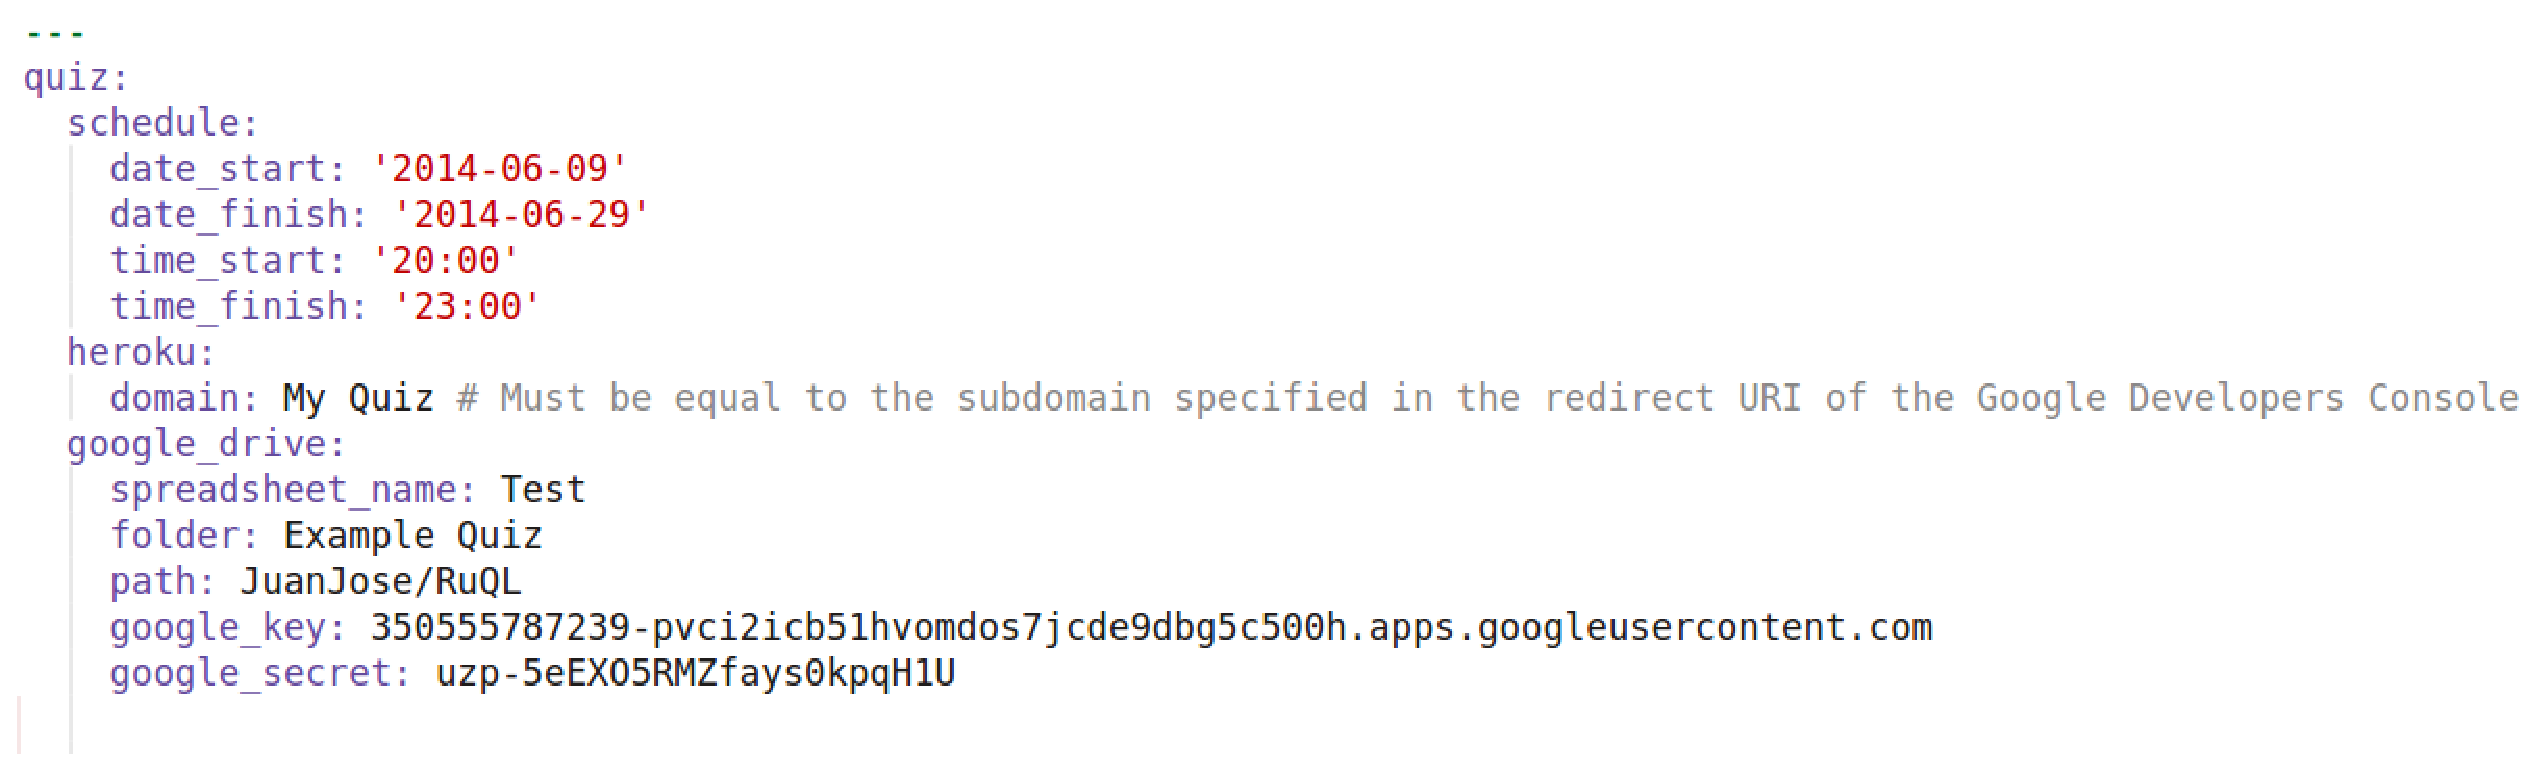
\includegraphics[width=1.2\textwidth]{images/config_yml.eps}
\caption{Ejemplo de fichero \textit{config.yml} con la informaci\'on necesaria}
\label{fig:config_yml}
\end{center}
\end{figure}
\newpage

Para a\~{n}adir este fichero al fichero del cuestionario especificamos el path del fichero en notaci\'on de \ceis{s\'{\i}mbolo}:
\begin{verbatim}
  quiz 'Example quiz' do
    
    .
    .
    
    config :'examples/config.yml'
    .
    .
  end
\end{verbatim}
\newpage

%---------------------------------------------------------------------------------
\subsection{Dar de alta una aplicaci\'on en Google Developers Console}
\label{subsec:Apendice2.13}

Pasos para dar de alta una aplicaci\'on en \ceit{Google Developers Console}:
\begin{enumerate}
  \item Dirigirse a \href{https://console.developers.google.com/}{Google Developers Console}
  
  \item Crear un nuevo proyecto.
  \begin{figure}[H]
  \begin{center}
  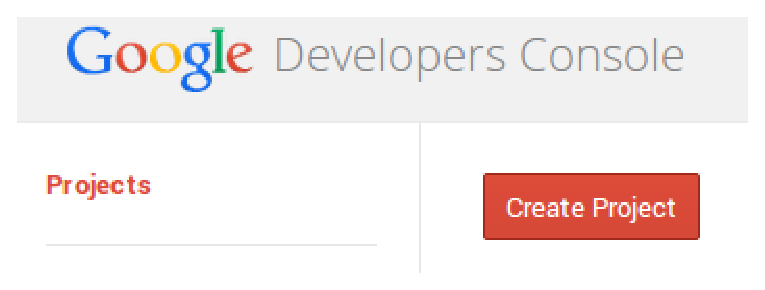
\includegraphics[width=0.5\textwidth]{images/gdc0.eps}
  \caption{Bot\'on para crear un nuevo proyecto}
  \label{fig:gdc0}
  \end{center}
  \end{figure}
  
  \item Elegir un nombre para el proyecto.
  \begin{figure}[!th]
  \begin{center}
  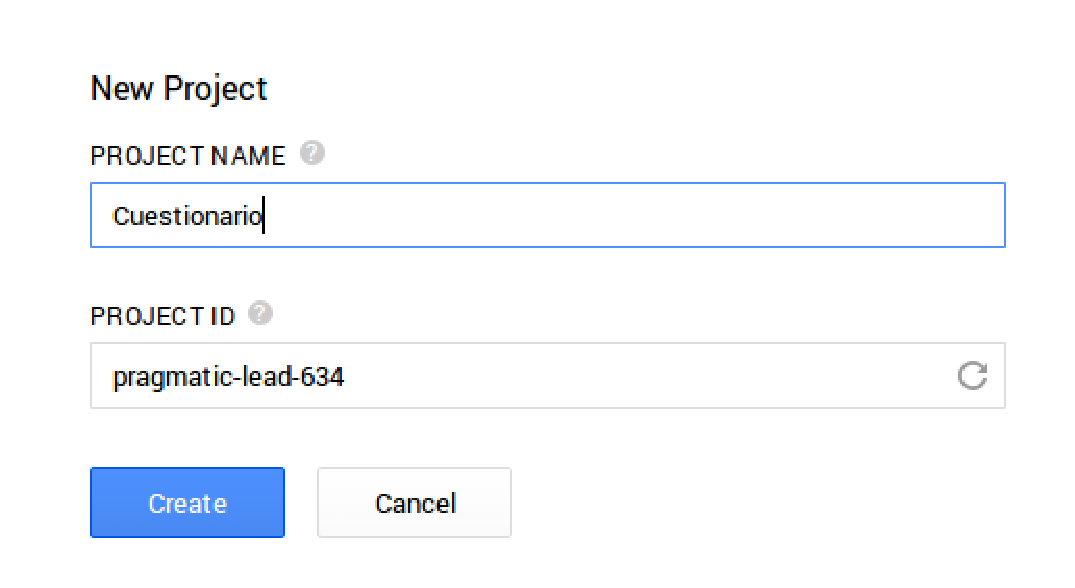
\includegraphics[width=0.7\textwidth]{images/gdc1.eps}
  \caption{Elegir nombre para el proyecto}
  \label{fig:gdc1}
  \end{center}
  \end{figure}
  \newpage
  
  \item Una vez se ha creado, se nos redireccionar\'a al mismo. Pinchamos en la secci\'on {\bfseries APIS \& AUTH} y elegimos la opci\'on \textit{APIs}.
  \begin{figure}[!th]
  \begin{center}
  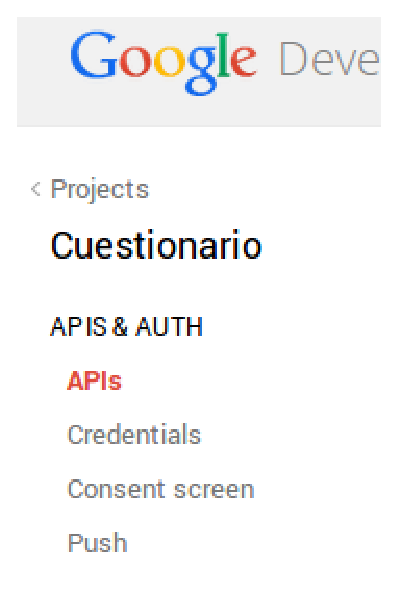
\includegraphics[width=0.3\textwidth]{images/gdc2.eps}
  \caption{Apartado de APIs}
  \label{fig:gdc2}
  \end{center}
  \end{figure}
    
  Deberemos activar las siguientes APIs:
  \begin{enumerate}
    \item \textit{Contacts API}
    \item \textit{Drive API}
    \item \textit{Drive SDK}
    \item \textit{Google+ API}
  \end{enumerate}
  \newpage
  
  \item Una vez hecho esto, nos iremos al apartado \textit{Credentials} dentro de {\bfseries APIS \& AUTH} y seleccionaremos \textit{Create new Client ID}.
  \begin{figure}[!th]
  \begin{center}
  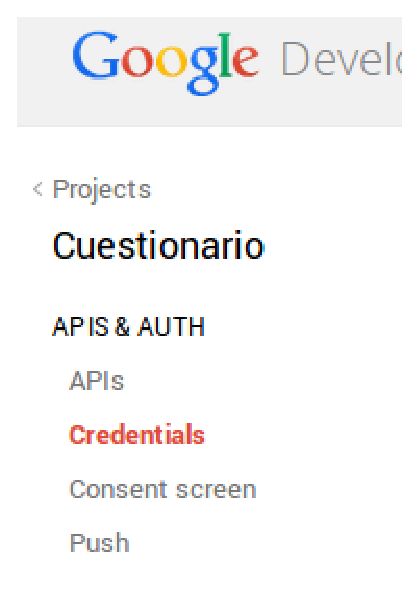
\includegraphics[width=0.3\textwidth]{images/gdc3.eps}
  \caption{Apartado de credenciales}
  \label{fig:gdc3}
  \end{center}
  \end{figure}
  
  \begin{figure}[!th]
  \begin{center}
  
\includegraphics[width=0.5\textwidth]{images/gdc4.eps}
  \caption{Crear nuevo cliente ID}
  \label{fig:gdc4}
  \end{center}
  \end{figure}
  \newpage
  
  \item Seleccionamos \textit{Web application} y establecemos la \ceit{URI} a la que \ceit{Google} debe devolvernos los datos. La URI debe ser igual a la de la imagen salvo
  en el subdominio de \ceit{Heroku}, en el que pondremos el que nos ha dado Heroku o el que hemos especificado en nuestro \textit{config.yml}
  \begin{figure}[!th]
  \begin{center}
  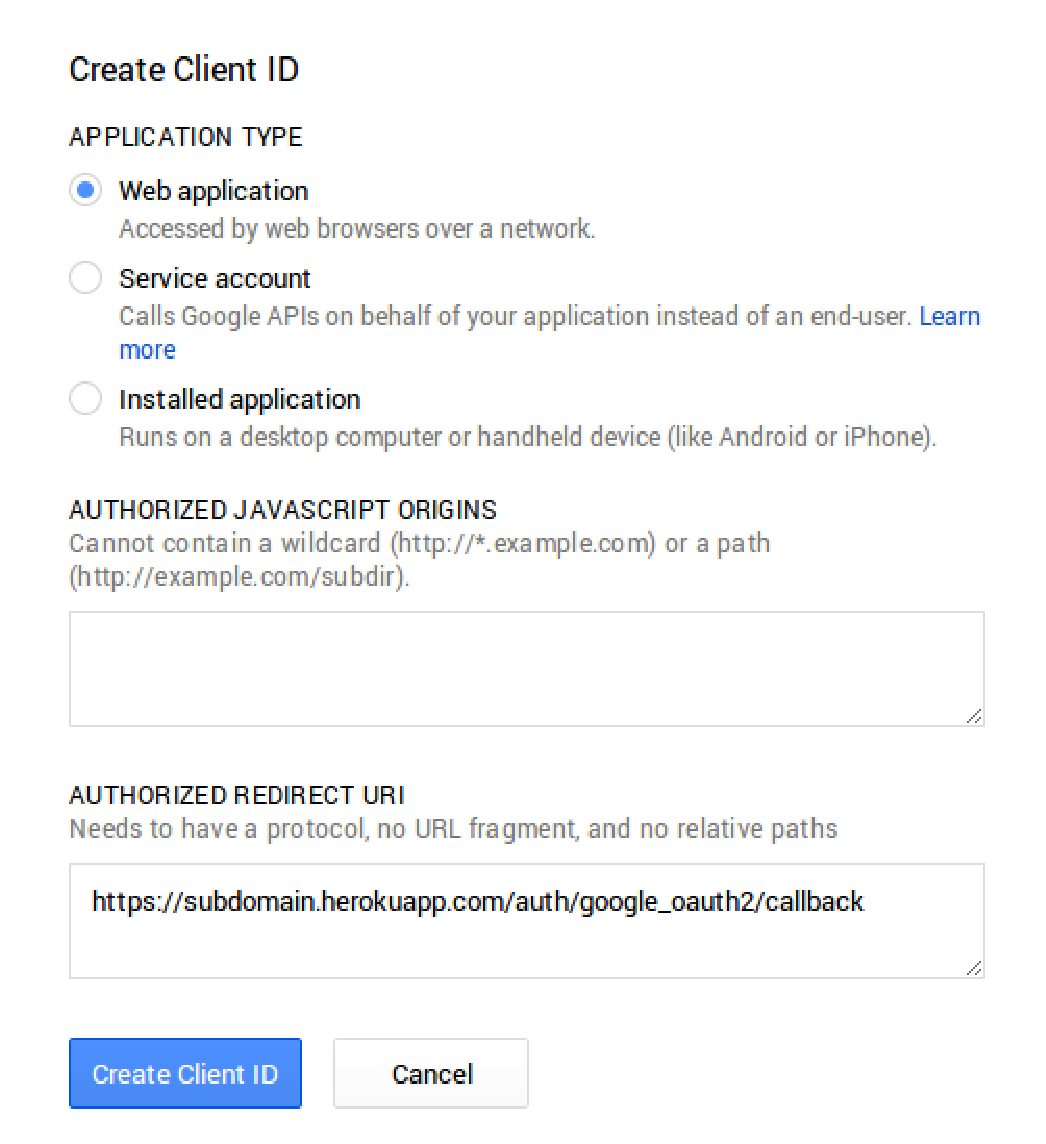
\includegraphics[width=0.7\textwidth]{images/gdc5.eps}
  \caption{Pantalla de creaci\'on del cliente ID}
  \label{fig:gdc5}
  \end{center}
  \end{figure}
  \newpage
  
  \item Opcionalmente, nos podemos dirigir al apartado \textit{Consent screen} dentro de {\bfseries APIS \& AUTH} para indicar el nombre que queremos que aparezca
  en la pantalla de permisos cuando alguien vaya a dar permiso a nuestra aplicaci\'on para que use sus datos. Adem\'as, se pueden a\~{n}adir otros campos tales como
  logos, URLs, etc.
  \begin{figure}[!th]
  \begin{center}
  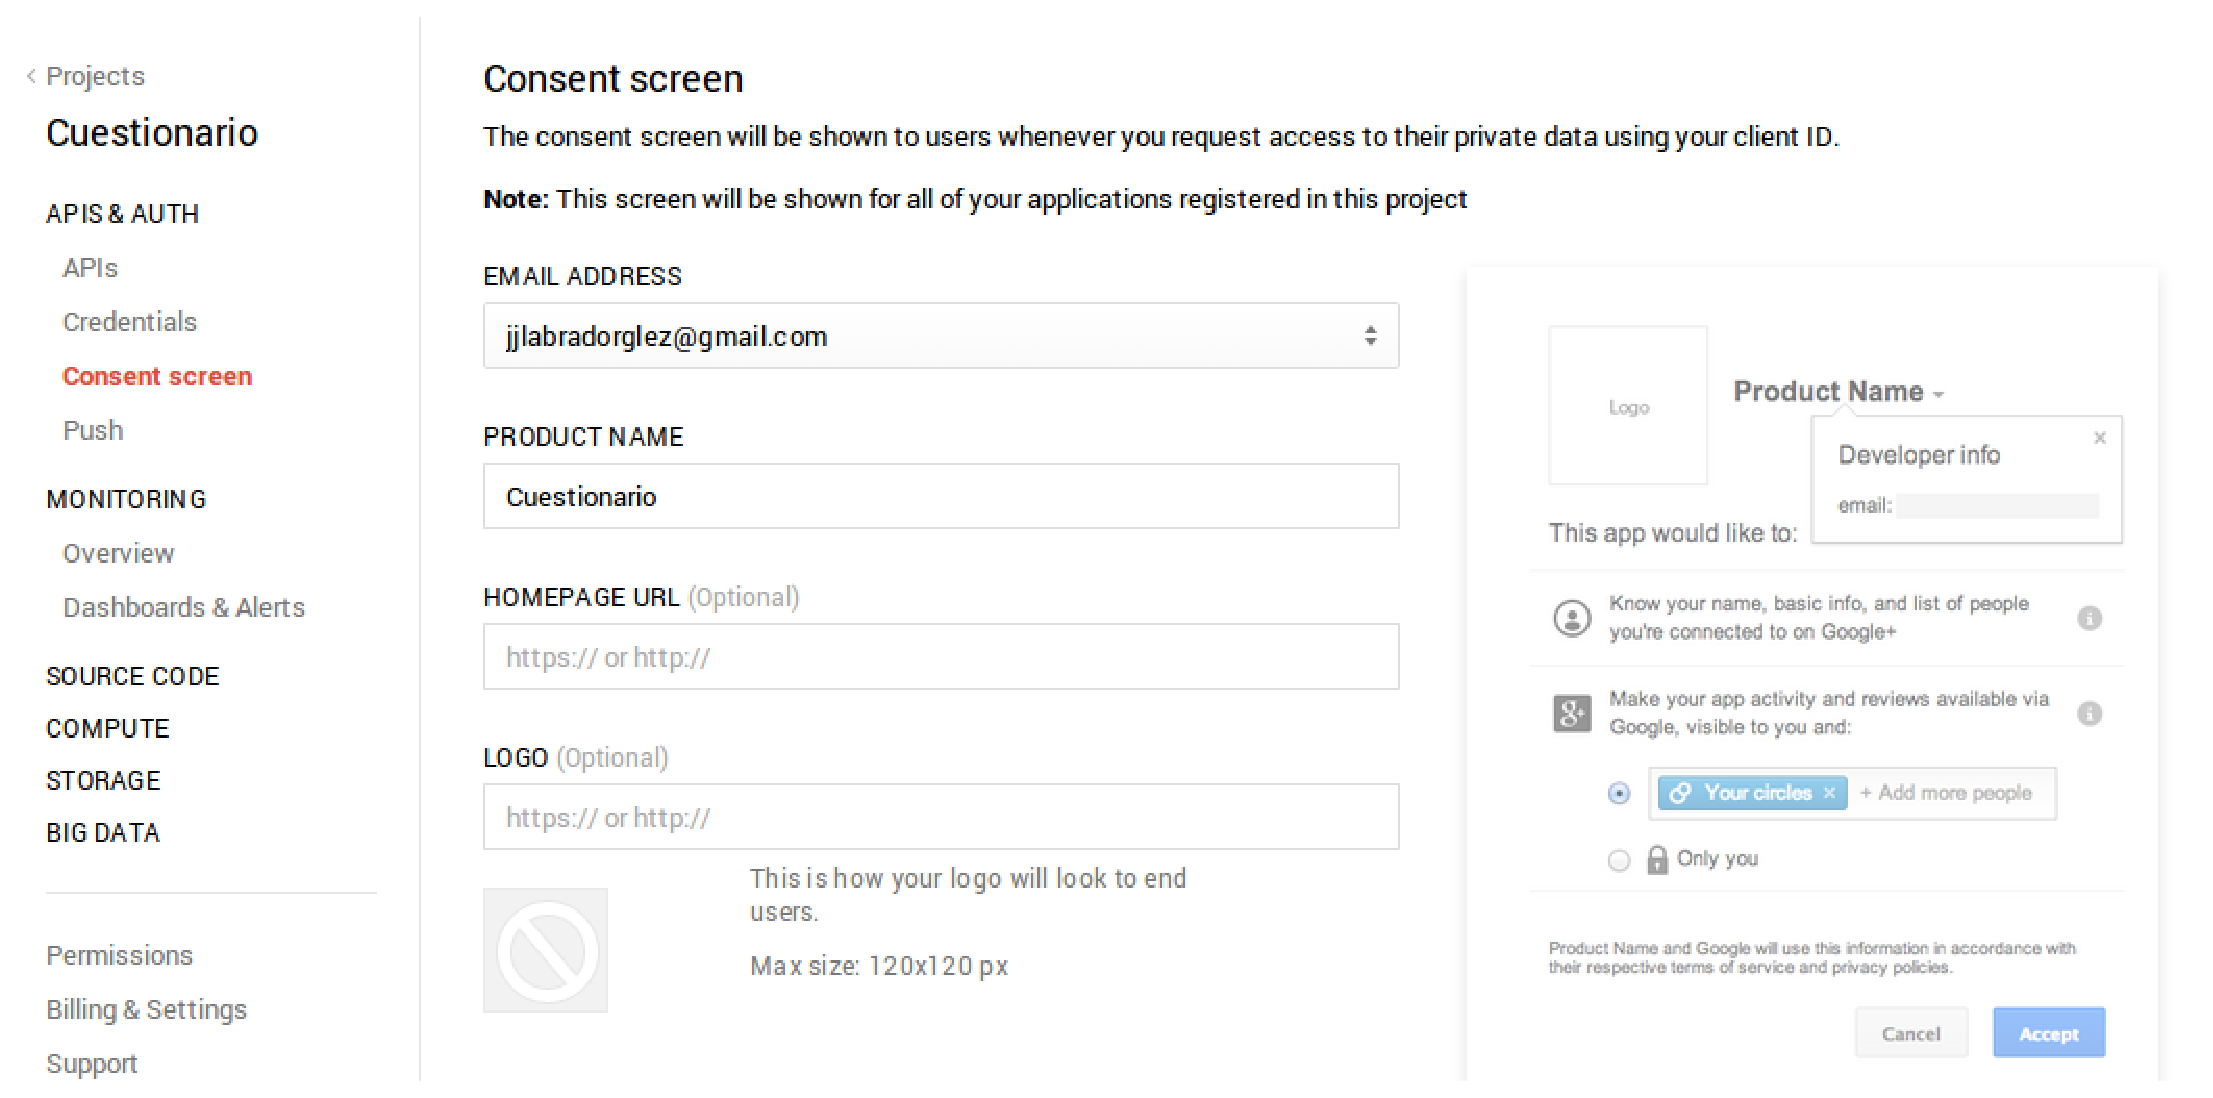
\includegraphics[width=1.2\textwidth]{images/gdc6.eps}
  \caption{Personalizar pantalla de permisos}
  \label{fig:gdc6}
  \end{center}
  \end{figure}
  
\end{enumerate}
\newpage

%---------------------------------------------------------------------------------
\subsection{Generando la aplicaci\'on}
\label{subsec:Apendice2.14}

Para generar la \ceit{aplicaci\'on}, ejecutamos el siguiente comando. Para este renderer es obligatorio el uso de alg\'un template:
\begin{verbatim}
[~]$ ruql [ruta_fichero_rb] Sinatra -t [ruta_template.html.erb]
\end{verbatim}

%---------------------------------------------------------------------------------
\subsection{Ficheros y directorios generados por el renderer}
\label{subsec:Apendice2.15}

Finalmente, los ficheros que genera este renderer son:
\begin{itemize}
  \item El c\'odigo Ruby del servidor ({\bfseries app.rb}).
  \item Un fichero {\bfseries config.ru} para la ejecuci\'on de la aplicaci\'on.
  \item Las vistas necesarias de la aplicaci\'on (incluyendo el cuestionario generado en HTML y un \ceit{template} \ceit{ERB} que se usar\'a para crear las copias de los cuestionarios
  realizados por los alumnos).
  \item Un \ceis{Gemfile} con las dependencias necesarias.
  \item Un \ceis{Rakefile} para automatizar tareas (de ejecuci\'on y despliegue de la aplicaci\'on).
  \item Una carpeta denominada \textit{config} con los datos de alumnos, profesores, las preguntas y respuestas y una copia del fichero \textit{config.yml}
  del cual se hara una lectura de los par\'ametros. De este modo, evitamos que las variables existentes en el c\'odigo contengan la informaci\'on sensible.
\end{itemize}
\newpage

%---------------------------------------------------------------------------------
\subsection{Ejecutando la aplicaci\'on}
\label{subsec:Apendice2.16}

En esta secci\'on se explicar\'a visualmente las funciones que realiza la aplicaci\'on:
\begin{enumerate}
  \item Si el alumno visita el cuestionario antes de que est\'e abierto, ver\'a la siguiente p\'agina:
  \begin{figure}[!th]
  \begin{center}
  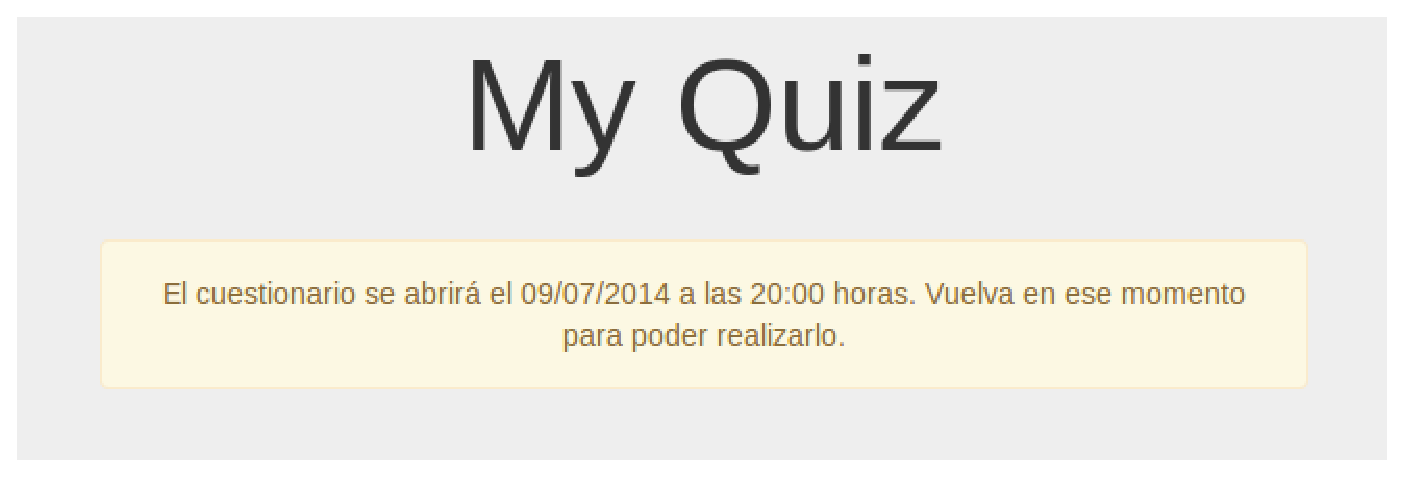
\includegraphics[width=0.9\textwidth]{images/app1.eps}
  \caption{Mensaje anunciando que el cuestionario no est\'a abierto}
  \label{fig:app1}
  \end{center}
  \end{figure}
  
  \item Si el alumno visita el cuestionario despu\'es de que se haya cerrado, ver\'a la siguiente p\'agina:
  \begin{figure}[!th]
  \begin{center}
  
\includegraphics[width=0.9\textwidth]{images/app2.eps}
  \caption{Mensaje anunciando que el cuestionario est\'a cerrado}
  \label{fig:app2}
  \end{center}
  \end{figure}
  \newpage
  
  \item Tanto los alumnos como los profesores ver\'an esta p\'agina al iniciar sesi\'on:
  \begin{figure}[!th]
  \begin{center}
  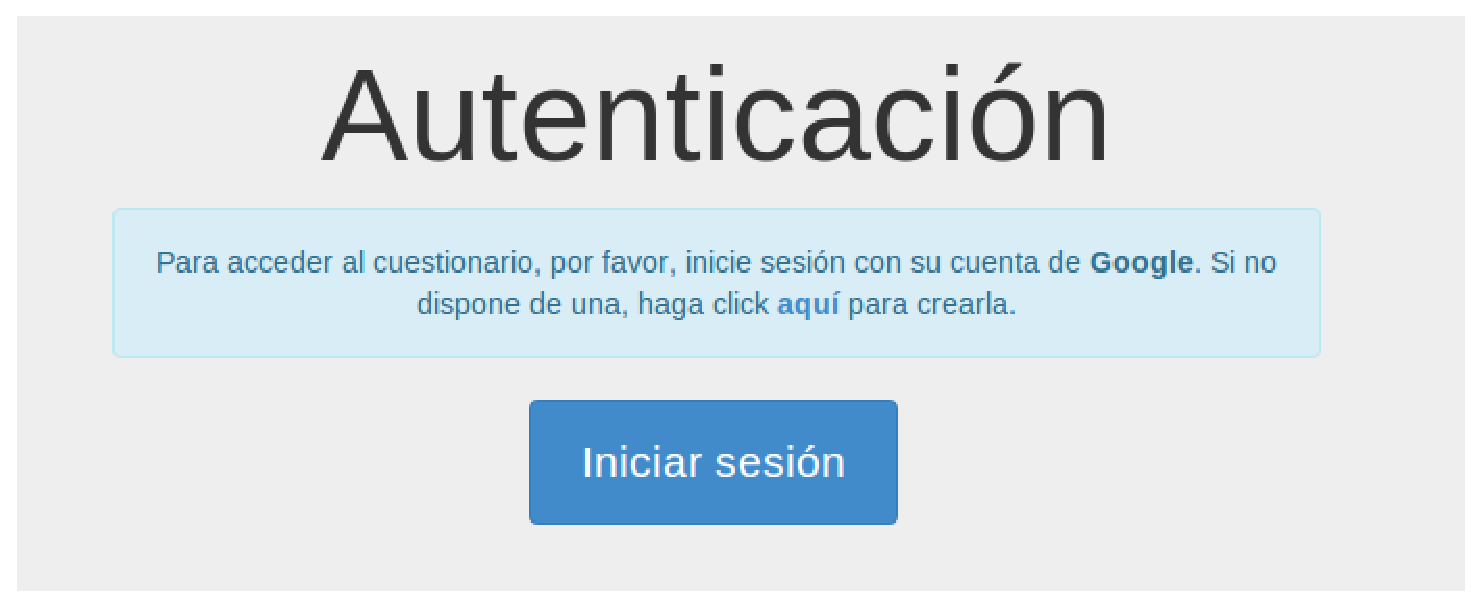
\includegraphics[width=0.9\textwidth]{images/app3.eps}
  \caption{P\'agina de iniciar sesi\'on}
  \label{fig:app3}
  \end{center}
  \end{figure}
  
  
  \item El profesor ver\'a esta p\'agina cuando vaya a activar el cuestionario:
  \begin{figure}[!th]
  \begin{center}
  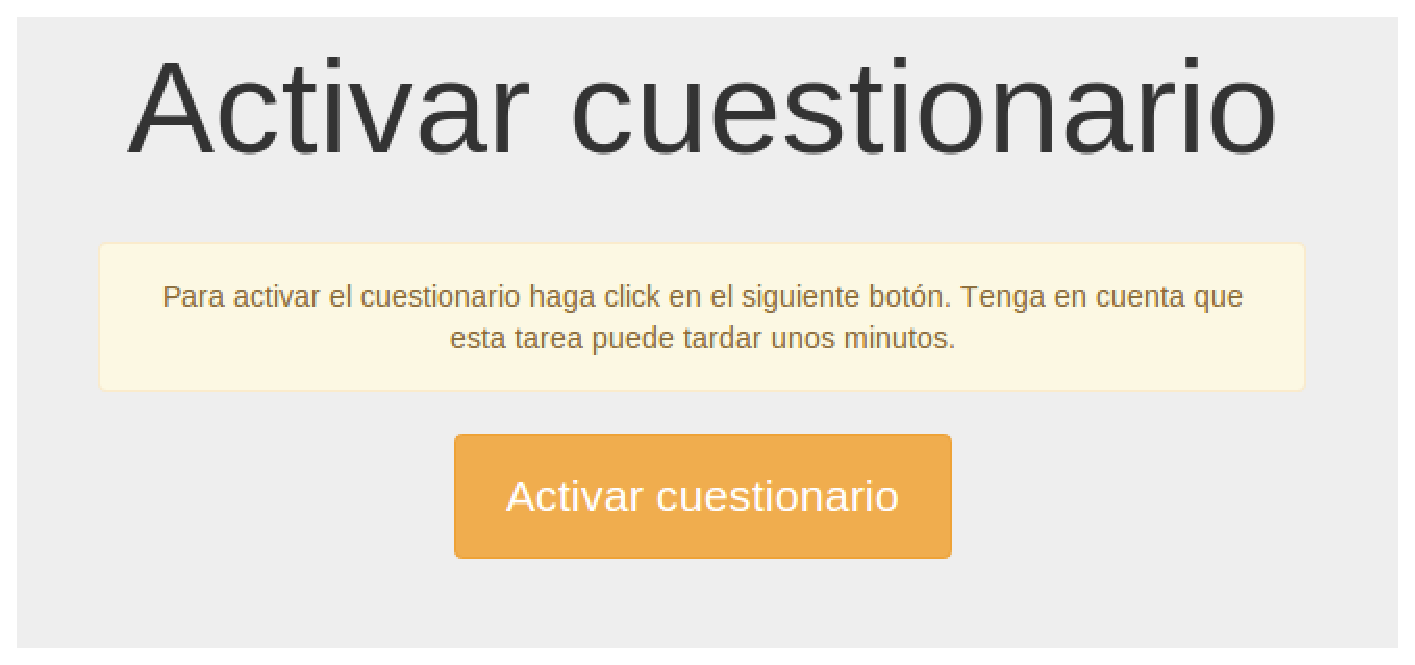
\includegraphics[width=0.75\textwidth]{images/app4.eps}
  \caption{P\'agina de activar cuestionario}
  \label{fig:app4}
  \end{center}
  \end{figure}
  \newpage
  
  \item Tanto los alumnos como los profesores ver\'an esta p\'agina para dar permisos a la aplicaci\'on al iniciar sesi\'on con \ceit{Google}:
  \begin{figure}[!th]
  \begin{center}
  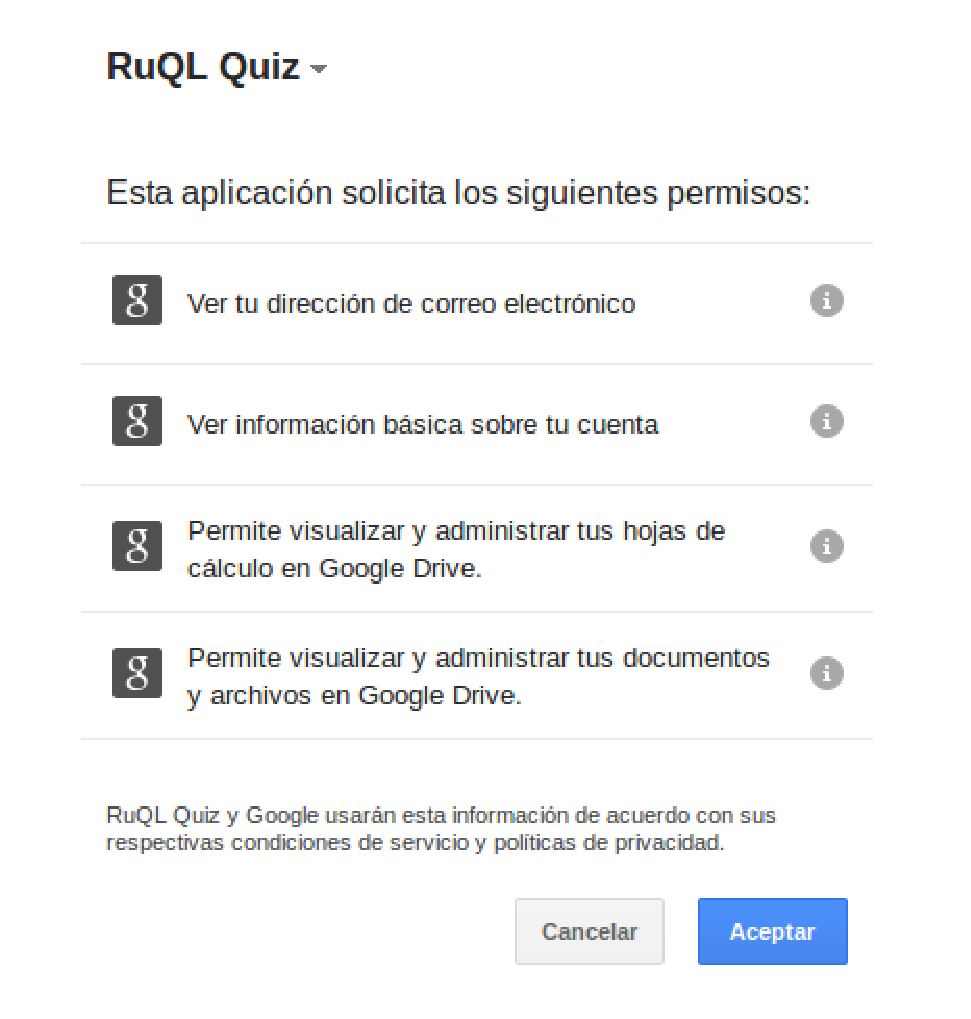
\includegraphics[width=0.6\textwidth]{images/app5.eps}
  \caption{P\'agina de dar permisos a la aplicaci\'on}
  \label{fig:app5}
  \end{center}
  \end{figure}
  
  \item Mientras el profesor no haya activado el \ceit{cuestionario}, los alumnos ver\'an esta p\'agina:
  \begin{figure}[!th]
  \begin{center}
  
\includegraphics[width=0.75\textwidth]{images/app6.eps}
  \caption{Mensaje anunciando que el cuestionario a\'un no est\'a activado}
  \label{fig:app6}
  \end{center}
  \end{figure}
  \newpage
  
  \item Cuando el profesor active el cuestionario ver\'a esta p\'agina. Puede ir a Google Drive para comprobar que la \ceit{hoja de c\'alculo} 
  se ha creado correctamente o visitar el cuestionario desplegado:
  \begin{figure}[!th]
  \begin{center}
  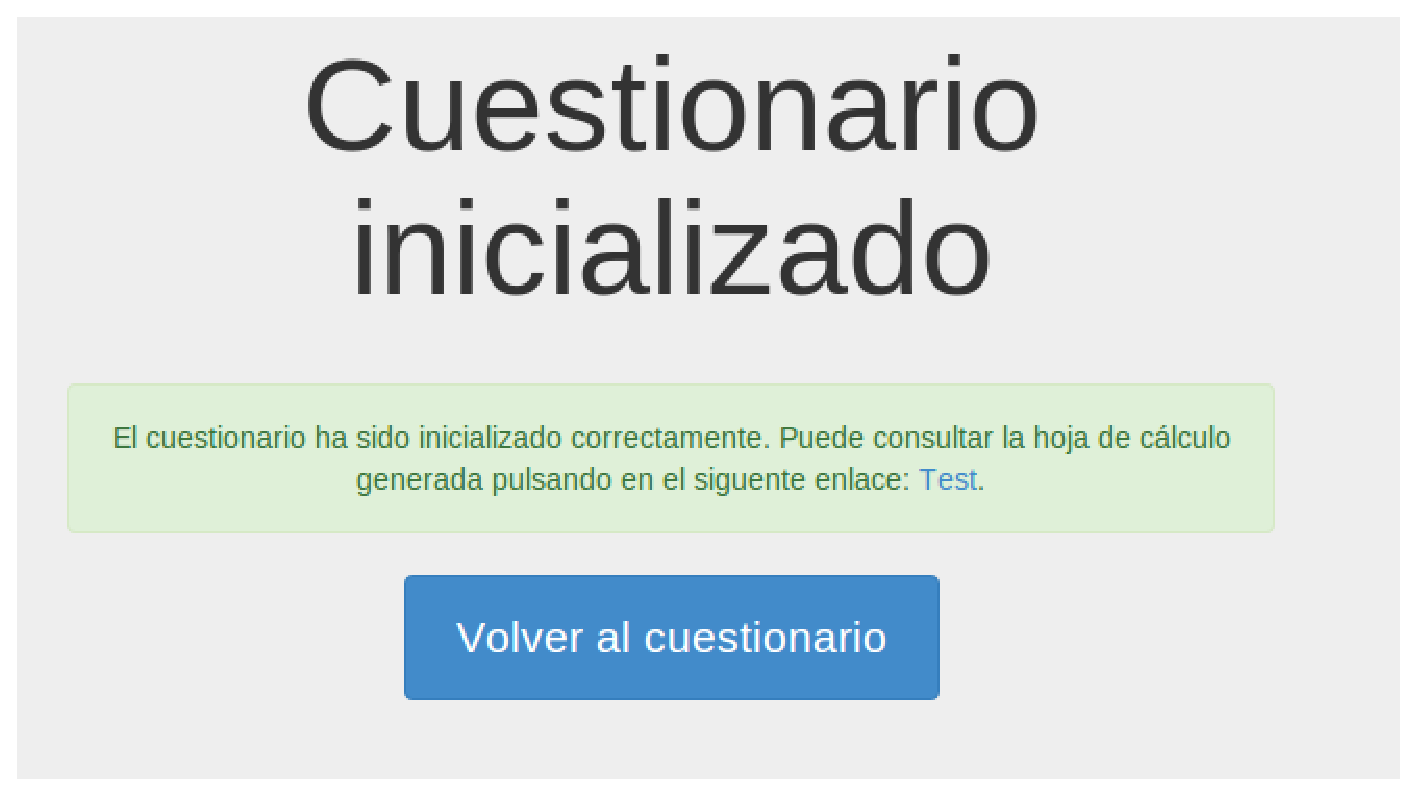
\includegraphics[width=0.8\textwidth]{images/app7.eps}
  \caption{Mensaje anunciando que el cuestionario ha activado}
  \label{fig:app7}
  \end{center}
  \end{figure}

  \item As\'{\i} se ver\'{\i}a el cuestionario desplegado:
  \begin{figure}[!th]
  \begin{center}
  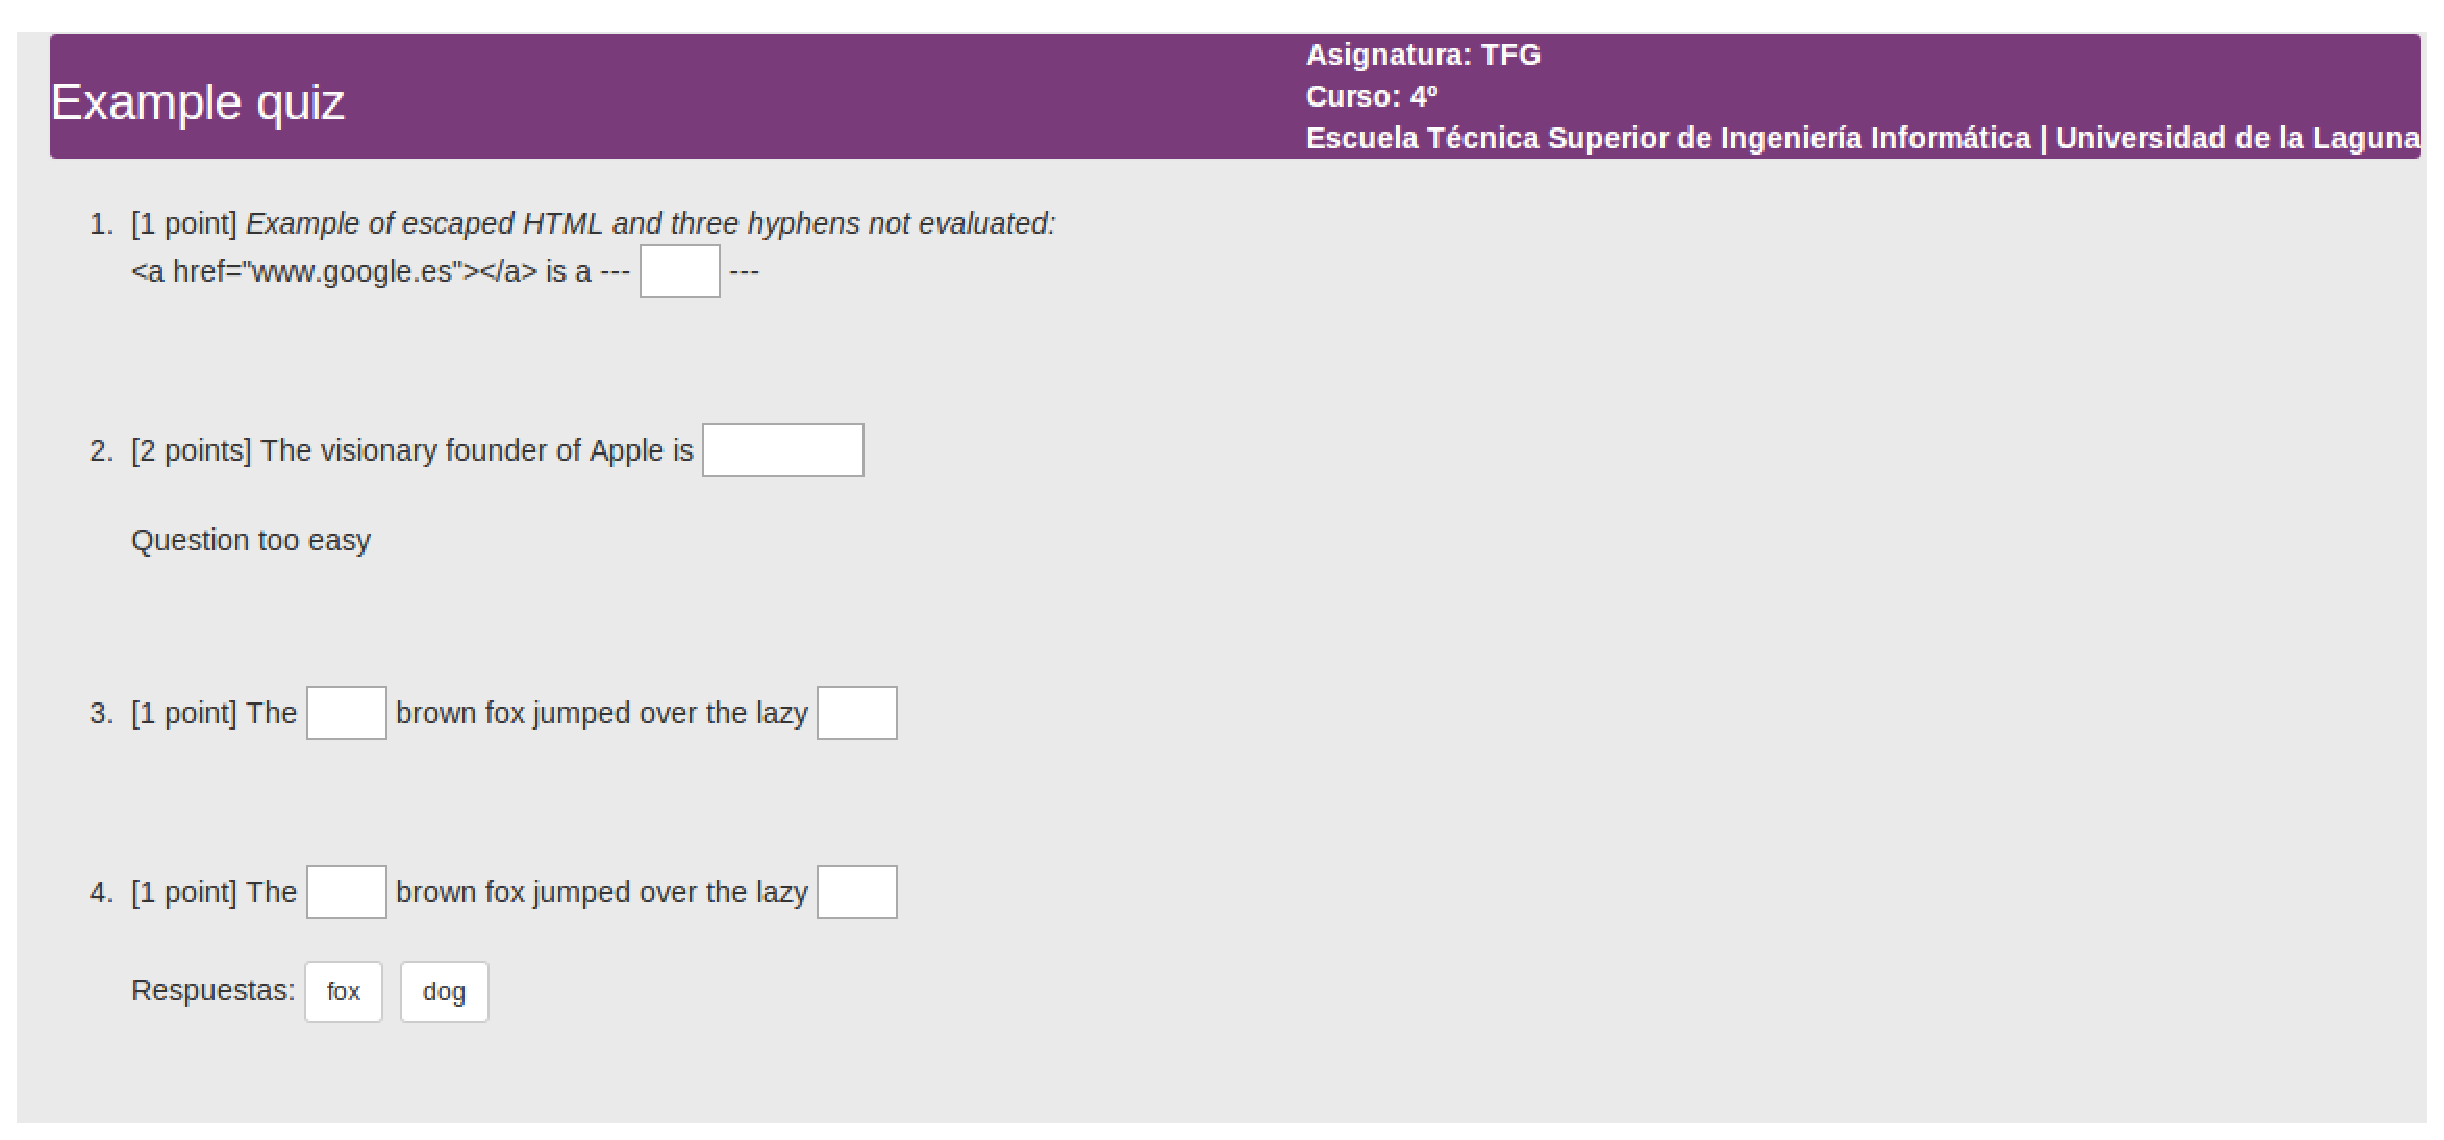
\includegraphics[width=1\textwidth]{images/app8.eps}
  \caption{Cuestionario desplegado}
  \label{fig:app8}
  \end{center}
  \end{figure}
  \newpage
  
  \item Cuando el profesor termine de comprobar el cuestionario y pulse \textit{Enviar}, ver\'a la siguiente pantalla, que le permitir\'a regresar al cuestionario o ver
  su carpeta de Google Drive.
  \begin{figure}[!th]
  \begin{center}
  
\includegraphics[width=0.8\textwidth]{images/app9.eps}
  \caption{Mensaje anunciando que ha finalizado la revisi\'on del cuestionario}
  \label{fig:app9}
  \end{center}
  \end{figure}

  \item Esto es lo que ver\'a el profesor en su carpeta de \ceit{Google Drive}.
  \begin{figure}[!th]
  \begin{center}
  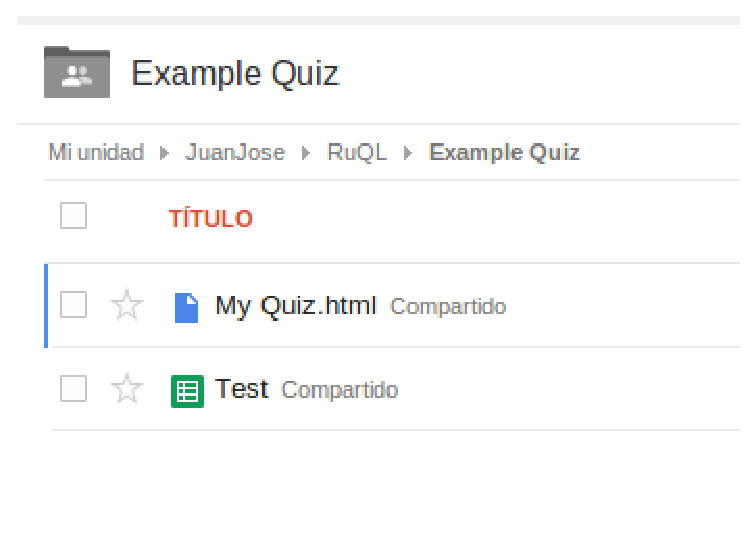
\includegraphics[width=0.6\textwidth]{images/app10.eps}
  \caption{Listado de ficheros dentro de la carpeta del cuestionario en Google Drive}
  \label{fig:app10}
  \end{center}
  \end{figure}
  \newpage

  \item Esta es la hoja de c\'alculo creada con toda la informaci\'on. Esta es la primera hoja, que contiene la informaci\'on de los alumnos.
  \begin{figure}[!th]
  \begin{center}
  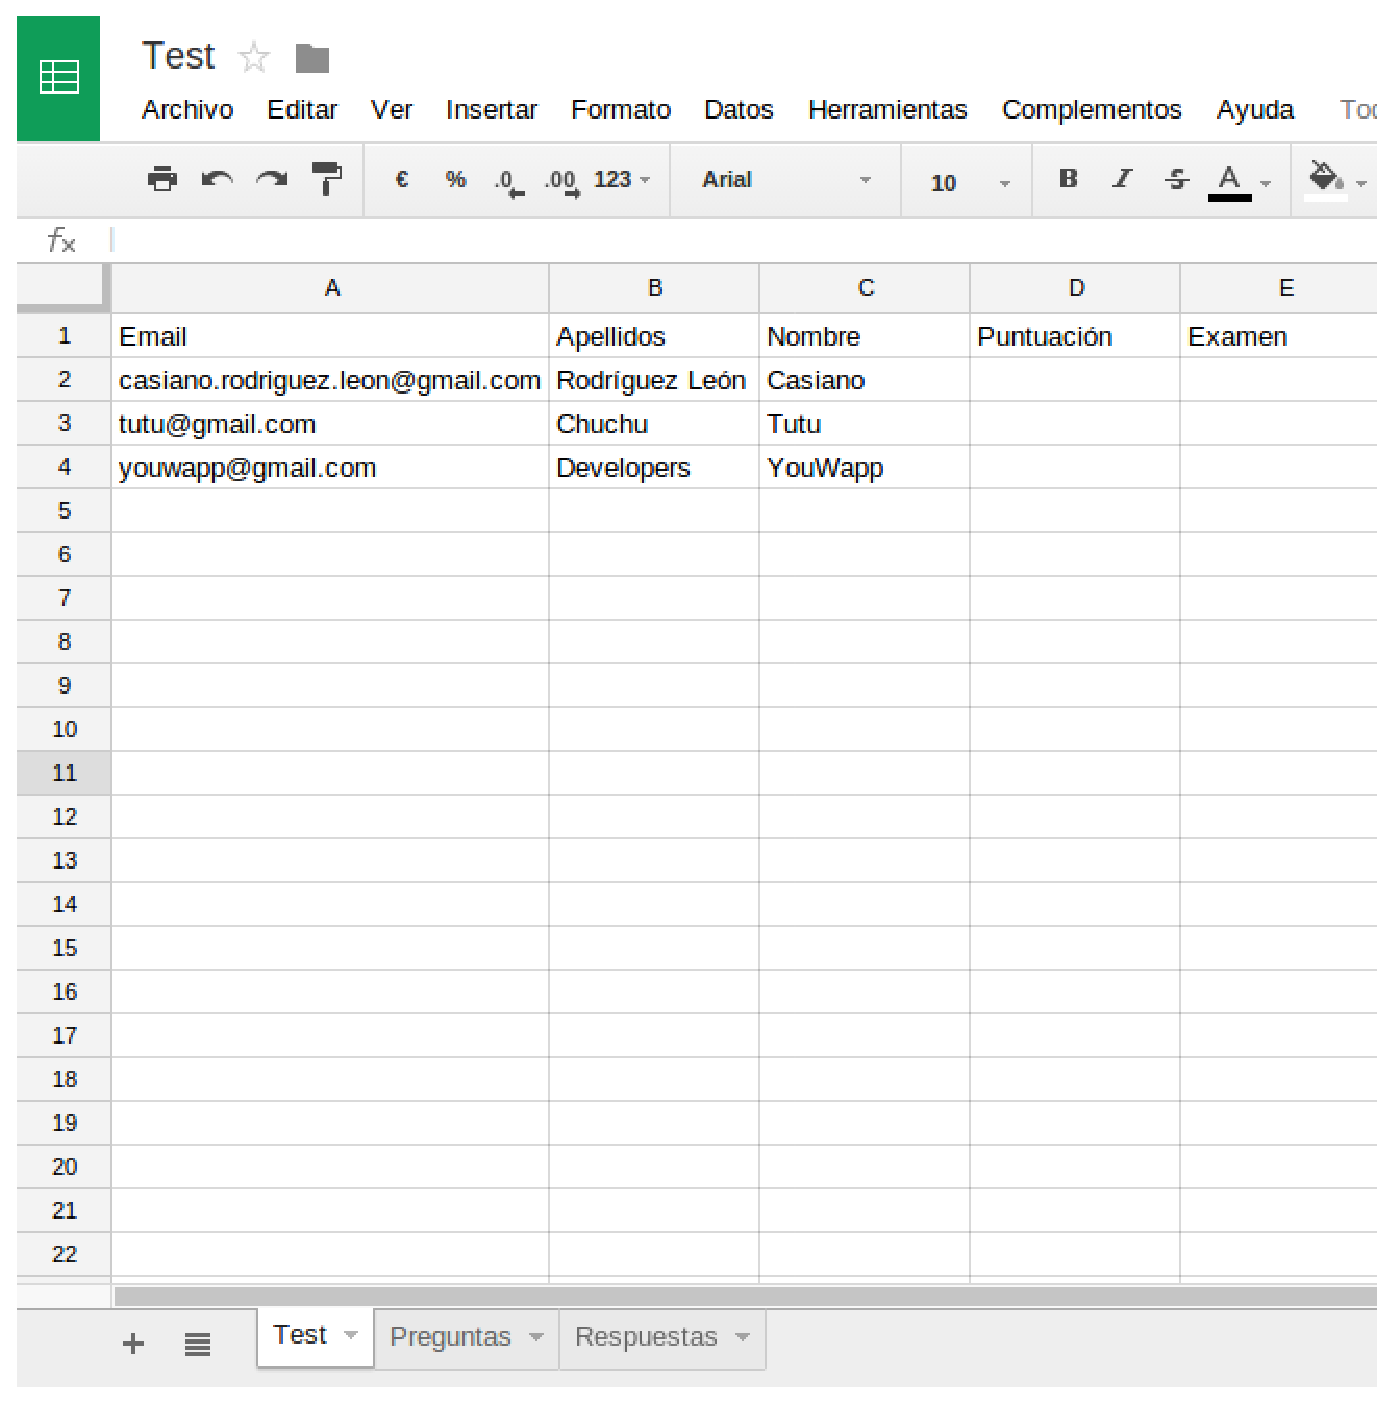
\includegraphics[width=1.1\textwidth]{images/app11.eps}
  \caption{Hoja de c\'alculo con la informaci\'on de los alumnos}
  \label{fig:app11}
  \end{center}
  \end{figure}
  \newpage
  
  \item Esta es la segunda hoja, que contiene la informaci\'on de las preguntas.
  \begin{figure}[!th]
  \begin{center}
  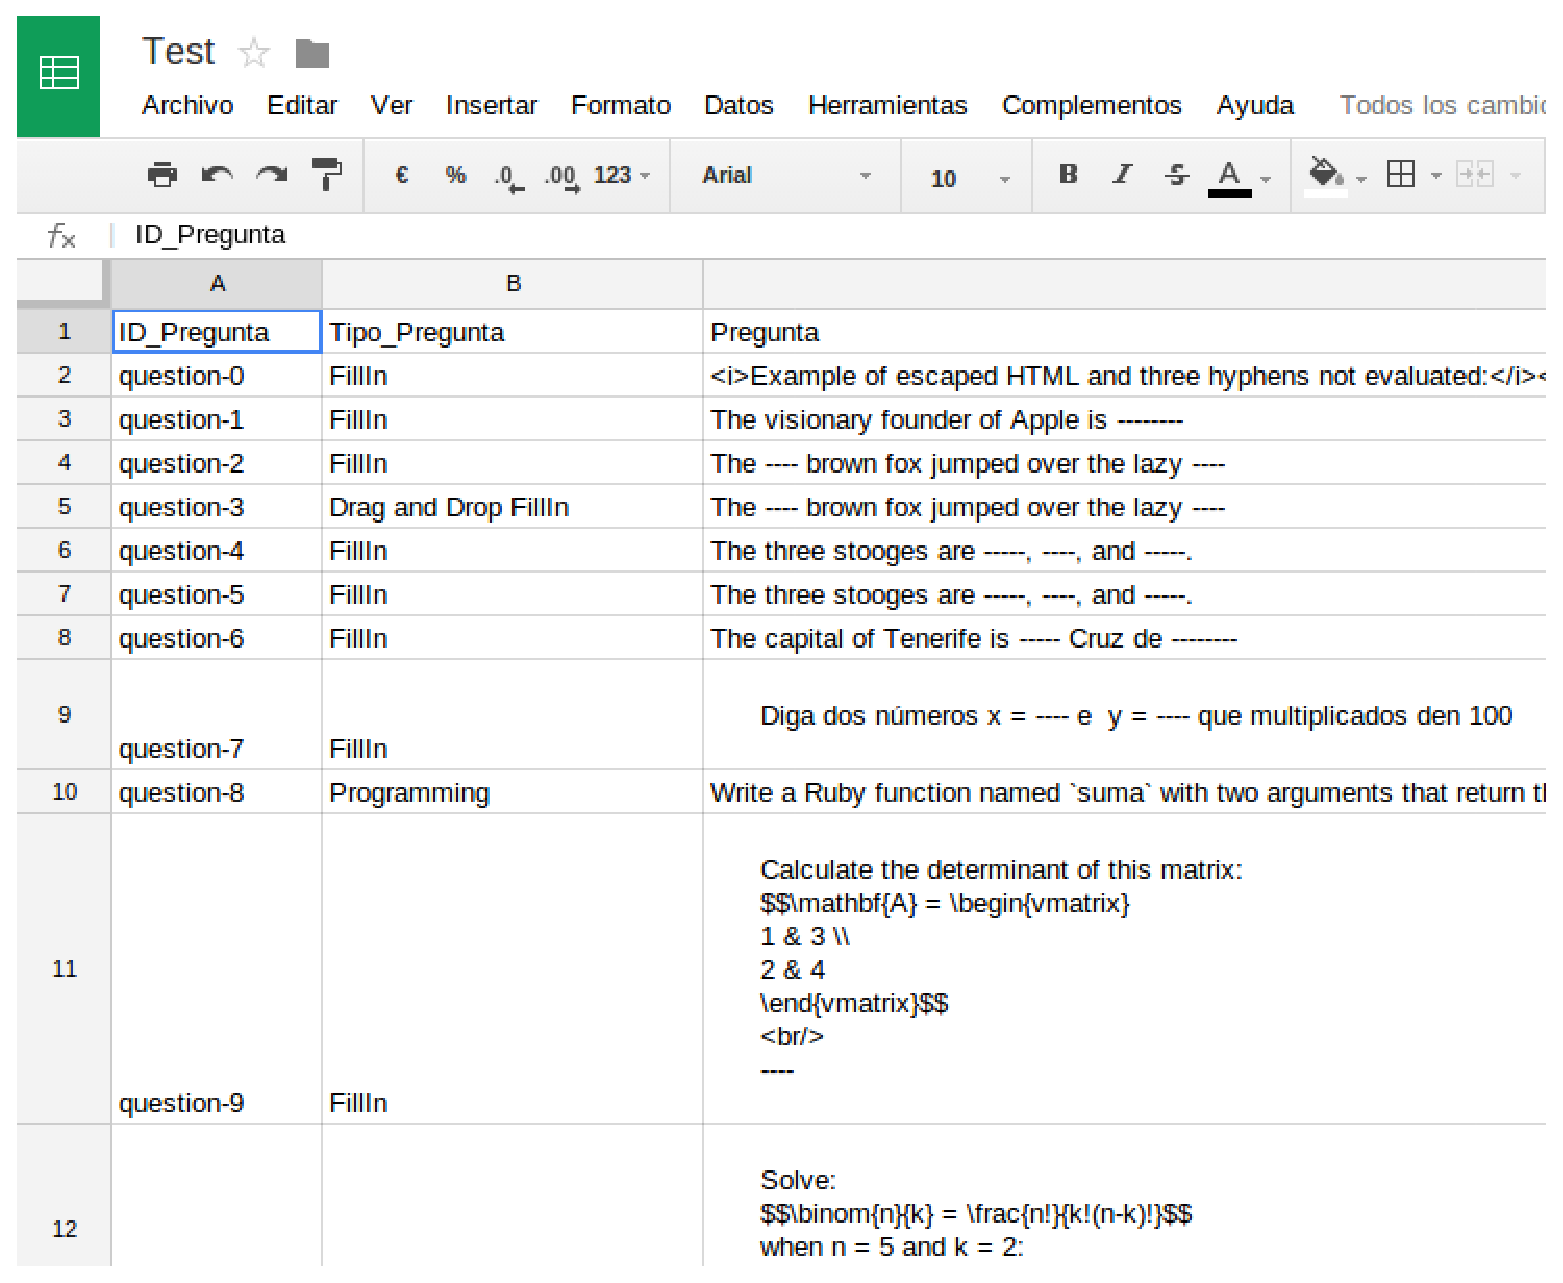
\includegraphics[width=1.1\textwidth]{images/app12.eps}
  \caption{Hoja de c\'alculo con la informaci\'on de las preguntas}
  \label{fig:app12}
  \end{center}
  \end{figure}
  \newpage

  \item Esta es la tercera hoja, que contiene la informaci\'on de las respuestas correctas.
  \begin{figure}[!th]
  \begin{center}
  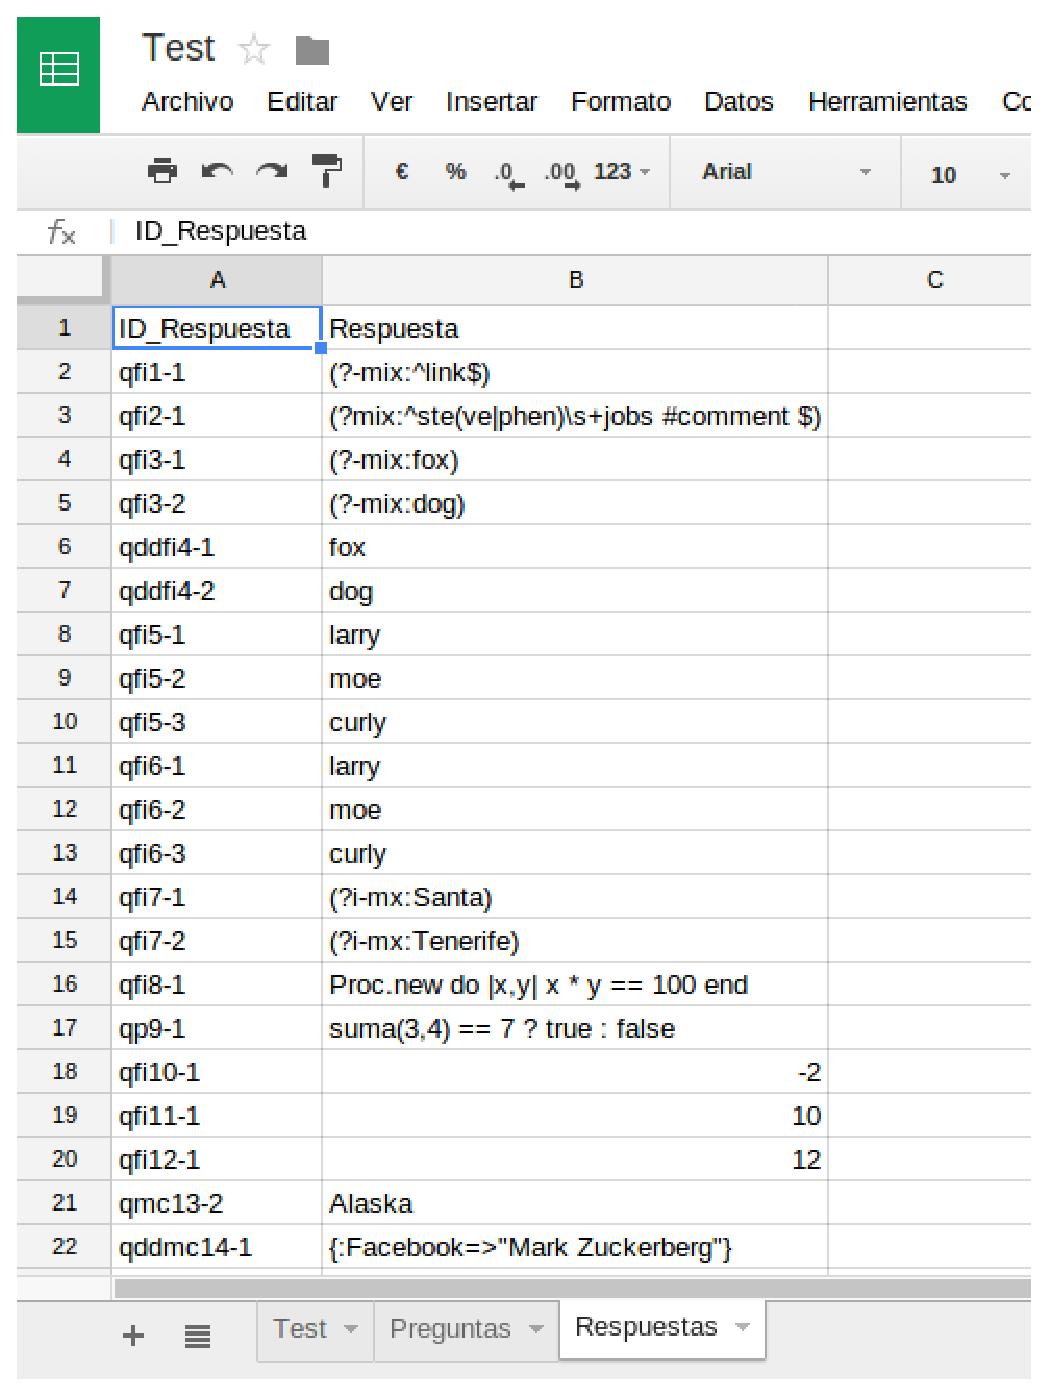
\includegraphics[width=0.8\textwidth]{images/app13.eps}
  \caption{Hoja de c\'alculo con la informaci\'on de las respuestas correctas}
  \label{fig:app13}
  \end{center}
  \end{figure}
  \newpage

  \item Cuando un alumno complete el cuestionario, ver\'a la siguiente pantalla. Podr\'a repetir el cuestionario todas las veces que desee dentro de la
  fecha permitida:
  \begin{figure}[!th]
  \begin{center}
  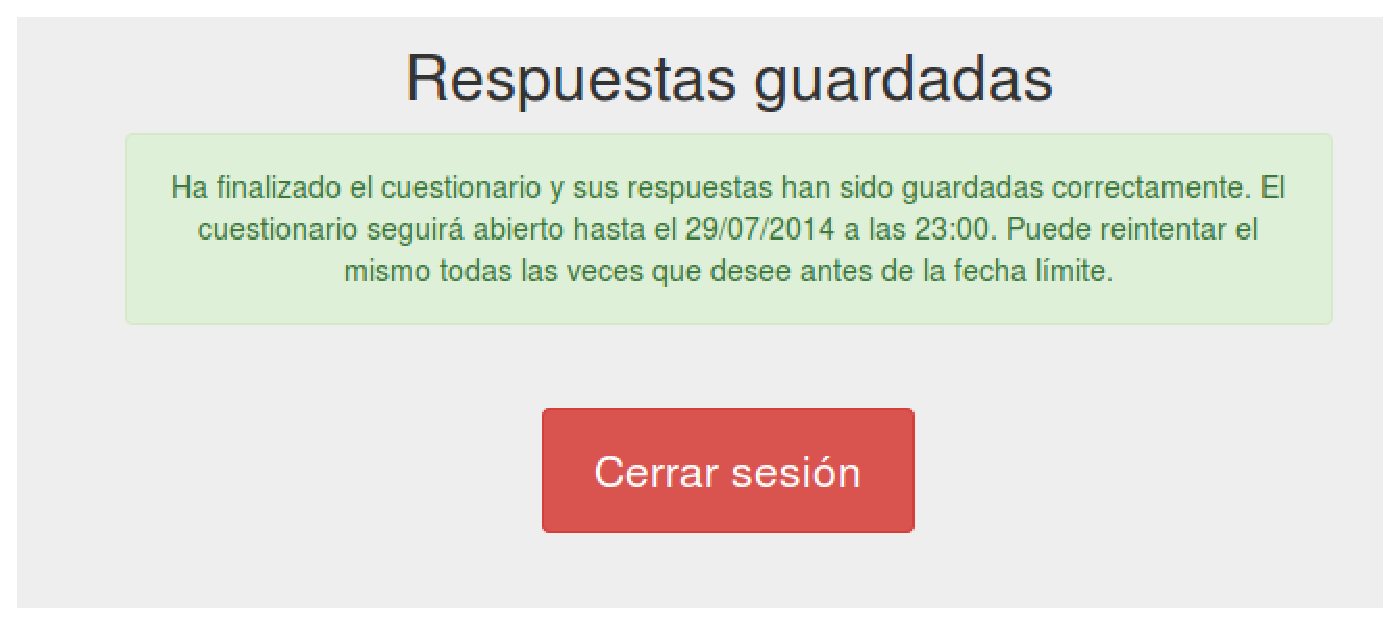
\includegraphics[width=1\textwidth]{images/app14.eps}
  \caption{Mensaje anunciando que ha completado cuestionario}
  \label{fig:app14}
  \end{center}
  \end{figure}
  \newpage
  
  \item Una vez completado el cuestionario, se crear\'a una nueva hoja dentro de la hoja de c\'alculo del profesor con la puntuaci\'on que ha
  sacado el alumno en cada pregunta:
  \begin{figure}[!th]
  \begin{center}
  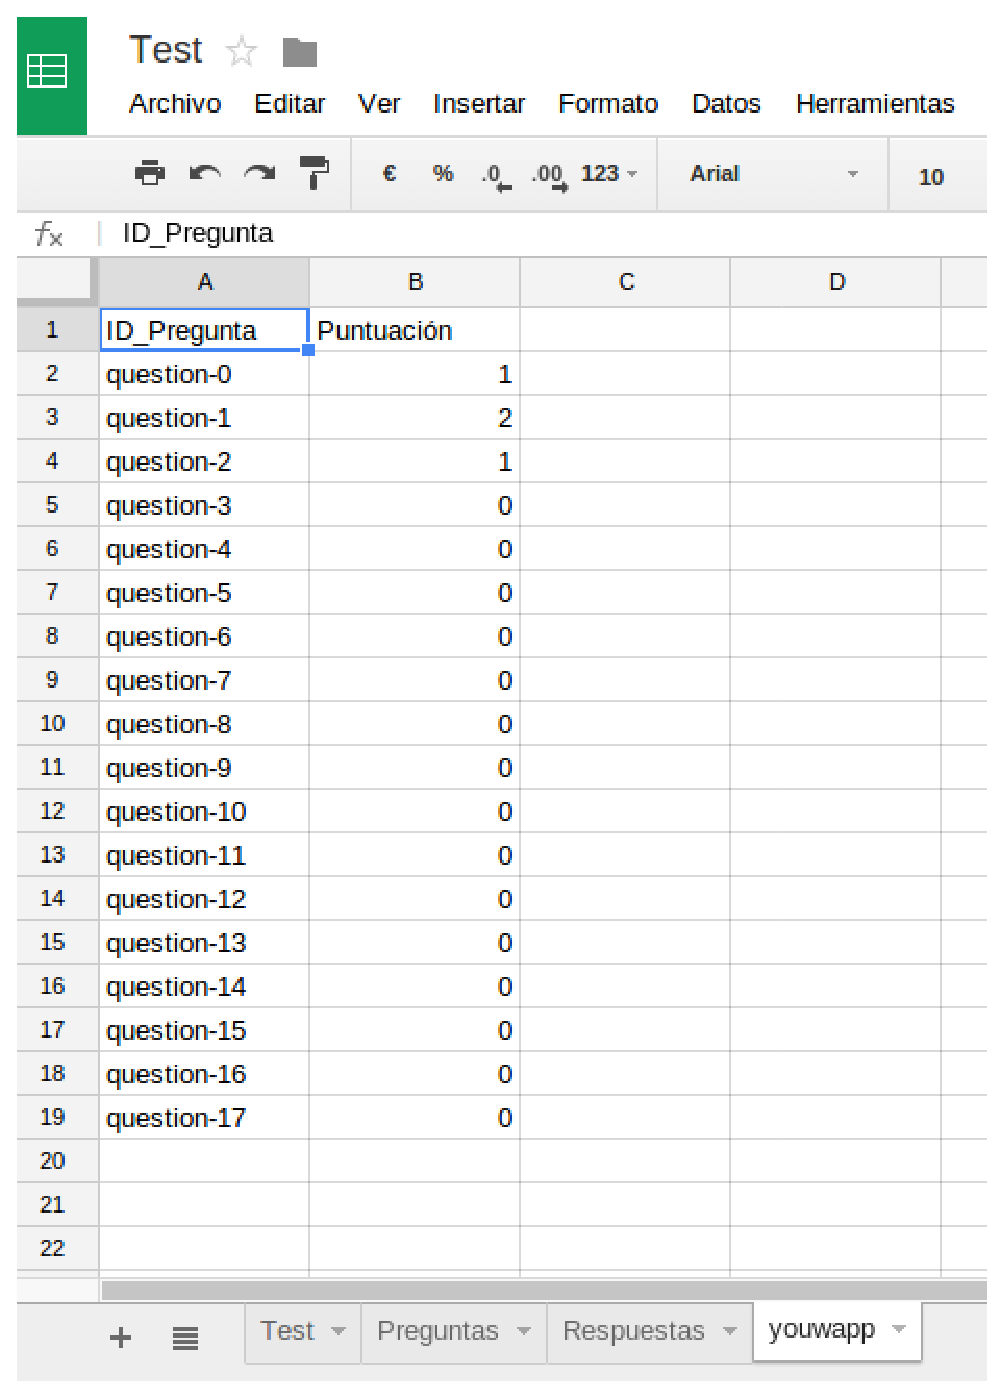
\includegraphics[width=0.8\textwidth]{images/app15.eps}
  \caption{Hoja de c\'alculo con la puntuaci\'on por preguntas}
  \label{fig:app15}
  \end{center}
  \end{figure}
  \newpage
  
  \item En la primera hoja, se a\~{n}adir\'a la informaci\'on del alumno que hizo el cuestionario, su nota y un enlace a la copia del \ceit{examen} que realiz\'o.
  \begin{figure}[!th]
  \begin{center}
  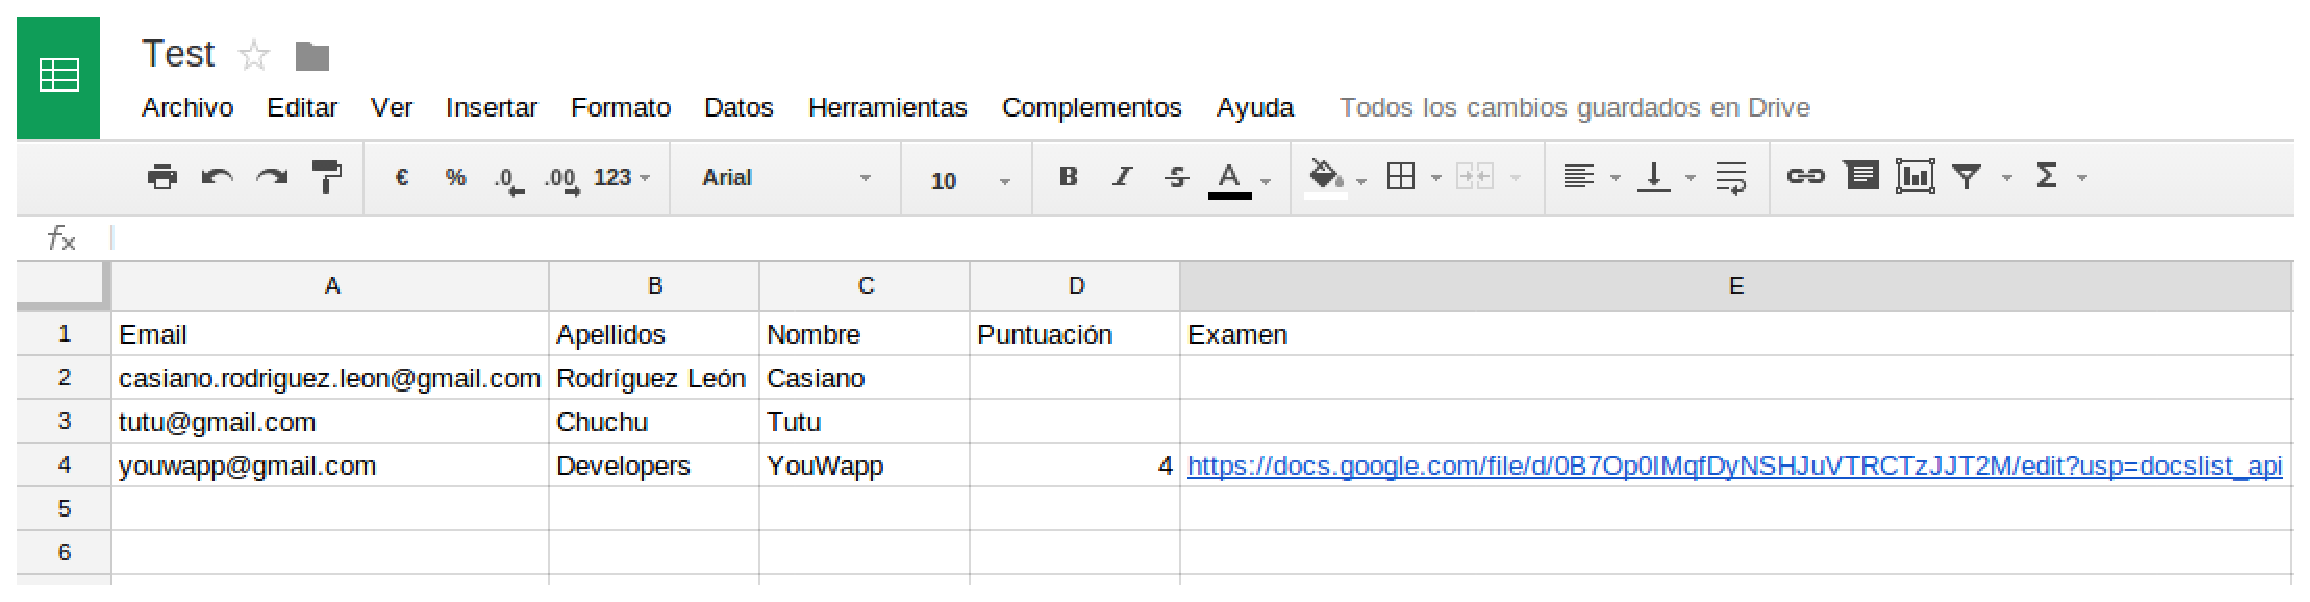
\includegraphics[width=1.1\textwidth]{images/app16.eps}
  \caption{Informaci\'on actualizada del alumno que realiz\'o el cuestionario}
  \label{fig:app16}
  \end{center}
  \end{figure}
  
  \item Dentro de la carpeta de Google Drive del profesor se crear\'a, adem\'as, una copia del cuestionario con las respuestas que puso el alumno.
  \begin{figure}[!th]
  \begin{center}
  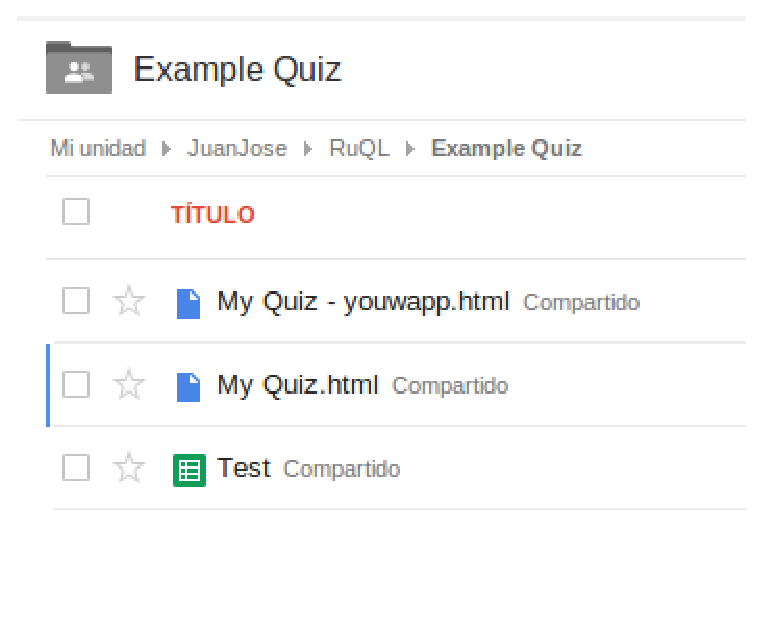
\includegraphics[width=0.6\textwidth]{images/app17.eps}
  \caption{Listado de ficheros en Google Drive con la copia hecha por el alumno}
  \label{fig:app17}
  \end{center}
  \end{figure}
  \newpage
  
  \item Por \'ultimo, esta ser\'{\i}a la copia del cuestionario generada con las respuestas del alumno:
  \begin{figure}[!th]
  \begin{center}
  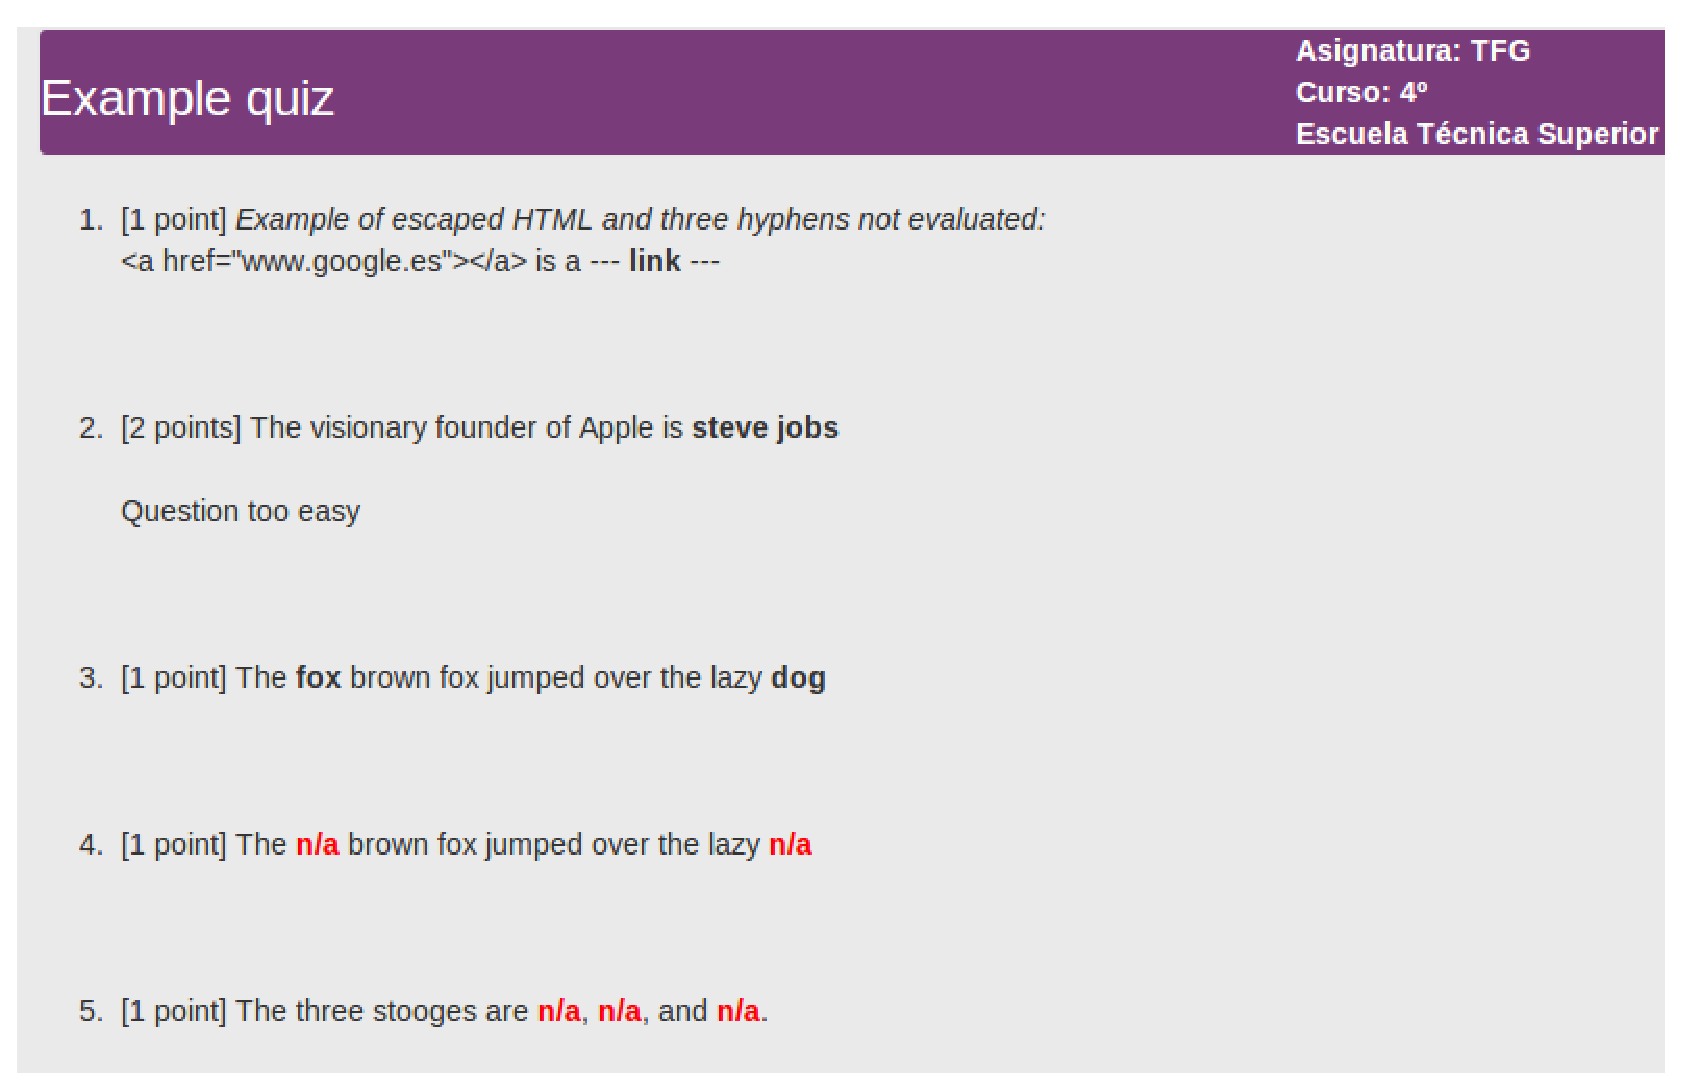
\includegraphics[width=1\textwidth]{images/app18.eps}
  \caption{Copia del cuestionario con las respuestas del alumno}
  \label{fig:app18}
  \end{center}
  \end{figure}
  
\end{enumerate}

%---------------------------------------------------------------------------------
\subsection{Otras consideraciones}
\label{subsec:Apendice2.17}

\begin{itemize}
  \item Este renderer no permite la opci\'on de mostrar respuestas mientras se realiza el cuestionario.
  \item El \ceit{Local Storage} tambi\'en funciona en este renderer, sin embargo, al ser un \ceit{JavaScript}, el evento de guardado de respuestas se dispara al perder el foco
  el \ceit{input} o \ceit{textarea} en el que nos encontramos.
\end{itemize}

\end{appendix}

%%%%%%%%%%%%%%%%%%%%%%%%%%%%%%%%%%%%%%%%%%%%%%%%%%%%%%%%%%%%%%%%%%%%%%%%%%%%%%%
\addcontentsline{toc}{chapter}{Bibliograf�a}
\bibliographystyle{plain}

\bibliography{memtfg}
\nocite{*}

%%%%%%%%%%%%%%%%%%%%%%%%%%%%%%%%%%%%%%%%%%%%%%%%%%%%%%%%%%%%%%%%%%%%%%%%%%%%%%%

\end{document}
